\documentclass[10pt]{article}

%Math
\usepackage{amsmath}
\usepackage{amsfonts}
\usepackage{amssymb}
\usepackage{amsthm}
\usepackage{ulem}
\usepackage{stmaryrd} %f\UTF{00FC}r Blitz!

%PageStyle
\usepackage[ngerman]{babel} % deutsche Silbentrennung
\usepackage[utf8]{inputenc} 
\usepackage{fancyhdr, graphicx}
\usepackage[scaled=0.92]{helvet}
\usepackage{enumitem}
\usepackage{parskip}
\usepackage[a4paper,top=2cm]{geometry}
\setlength{\textwidth}{17cm}
\setlength{\oddsidemargin}{-0.5cm}


% Shortcommands
\newcommand{\Bold}[1]{\textbf{#1}} %Boldface
\newcommand{\Kursiv}[1]{\textit{#1}} %Italic
\newcommand{\T}[1]{\text{#1}} %Textmode
\newcommand{\Nicht}[1]{\T{\sout{$ #1 $}}} %Streicht Shit durch

%Arrows
\newcommand{\lra}{\leftrightarrow} 
\newcommand{\ra}{\rightarrow}
\newcommand{\la}{\leftarrow}
\newcommand{\lral}{\longleftrightarrow}
\newcommand{\ral}{\longrightarrow}
\newcommand{\lal}{\longleftarrow}
\newcommand{\Lra}{\Leftrightarrow}
\newcommand{\Ra}{\Rightarrow}
\newcommand{\La}{\Leftarrow}
\newcommand{\Lral}{\Longleftrightarrow}
\newcommand{\Ral}{\Longrightarrow}
\newcommand{\Lal}{\Longleftarrow}

\newcommand{\BN}{\mathfrak{B}} %Belegung
\newcommand{\RN}{\mathbb{R}} %Real Number
\newcommand{\NN}{\mathbb{N}} %Natural Number
\newcommand{\QN}{\mathbb{Q}} %Rational Number
\newcommand{\ZN}{\mathbb{Z}} %ganze Zahlen
\newcommand{\CN}{\mathbb{C}}

% Code listenings
\usepackage{color}
\usepackage{xcolor}
\usepackage{listings}
\usepackage{caption}
\DeclareCaptionFont{white}{\color{white}}
\DeclareCaptionFormat{listing}{\colorbox{gray}{\parbox{\textwidth}{#1#2#3}}}
\captionsetup[lstlisting]{format=listing,labelfont=white,textfont=white}
\lstdefinestyle{CStyle}{
 language=Java,
 basicstyle=\footnotesize\ttfamily, % Standardschrift
 numbers=left,               % Ort der Zeilennummern
 numberstyle=\tiny,          % Stil der Zeilennummern
 stepnumber=5,              % Abstand zwischen den Zeilennummern
 numbersep=5pt,              % Abstand der Nummern zum Text
 tabsize=2,                  % Groesse von Tabs
 extendedchars=true,         %
 breaklines=true,            % Zeilen werden Umgebrochen
 frame=b,         
 %commentstyle=\itshape\color{LightLime}, Was isch das? O_o
 %keywordstyle=\bfseries\color{DarkPurple}, und das O_o
 basicstyle=\footnotesize\ttfamily,
 stringstyle=\color[RGB]{42,0,255}\ttfamily, % Farbe der String
 keywordstyle=\color[RGB]{127,0,85}\ttfamily, % Farbe der Keywords
 commentstyle=\color[RGB]{63,127,95}\ttfamily, % Farbe des Kommentars
 showspaces=false,           % Leerzeichen anzeigen ?
 showtabs=false,             % Tabs anzeigen ?
 xleftmargin=17pt,
 framexleftmargin=17pt,
 framexrightmargin=5pt,
 framexbottommargin=4pt,
 showstringspaces=false      % Leerzeichen in Strings anzeigen ?        
}

%Config
\renewcommand{\headrulewidth}{0pt}
\setlength{\headheight}{15.2pt}

%Metadata
\fancyfoot[C]{If you use this documentation for a exam, you should offer a beer to the authors!}
\title{
	\vspace{5cm}
	Computergrafik
}
\author{Jan Fässler}
\date{5. Semester (HS 2013)}


% hier beginnt das Dokument
\begin{document}

% Titelbild
\maketitle
\thispagestyle{fancy}

\newpage

% Inhaltsverzeichnis
\pagenumbering{Roman}
\tableofcontents	  	


\newpage
\setcounter{page}{1}
\pagenumbering{arabic}

% Inhalt Start

\section{Mathematische Grundlagen}
\subsection{Euklidischer Raum}
\begin{itemize}
	\item OpenGL benutzt das rechtshändige Koordinatensystem. Direct3D oder der Raytracer POVRay benutzen das links-händige System.
	\item Nehmen Sie die rechte Hand, streckt den Daumen nach rechts, den Zeigefinger nach oben und den Mittelfinger nach vorne.
	\item Die Finger zeigen dabei in die positiven Richtungen der x-, y- und z-Achse.
	\item Die Drehwinkel werden im Gegenuhrzeigersinn 	gemessen.
\end{itemize}
\begin{center}
	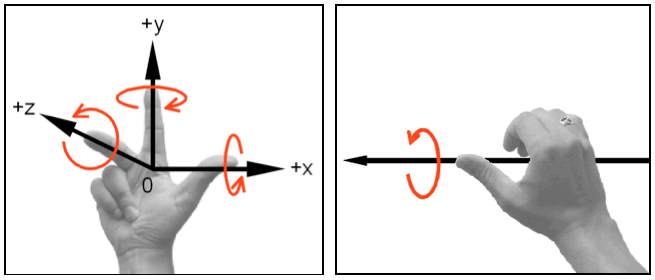
\includegraphics[scale=0.4]{euklidischer_raum.png}
\end{center}

\subsection{Vektoren}
\begin{itemize}
	\item Vektoren haben eine Richtung und eine Länge aber KEIN Ort.
	\item Punkte im Raum können durch Ortsvektoren beschrieben werden.
	\item Sie werden als n-Tupel, als geordnete Liste von reellen Zahlen beschrieben
	\item Punkte sind Orte, Vektoren sind Richtungen
\end{itemize}
\begin{center}
	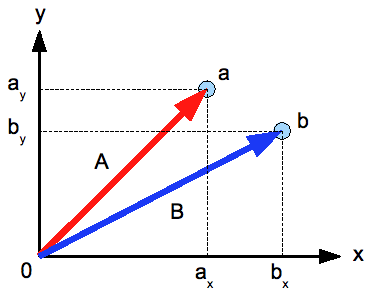
\includegraphics[scale=0.4]{vektoren.png}
\end{center}
\subsubsection{Addition}
\begin{equation}
	C=A+B=
	\begin{bmatrix}
	a_0+b_0 \\
	a_1+b_1 \\
	\dots \\
	 a_{n-1} + b_{n-1}
	\end{bmatrix}	
	\in \RN^n	
\end{equation}
\subsubsection{skalare Multiplikation}
\begin{equation}
	s*A=
	\begin{bmatrix}
	s*a_0 \\
	s*a_1 \\
	\dots \\
	s*a_{n-1}
	\end{bmatrix}
	\in \RN^n
\end{equation}
\subsubsection{Betrag}
\begin{equation}
	\text{Länge}=|A|=\sqrt{A * A} = \sqrt{a_0^2+a_1^2+\dots+a_{n-1}^2}
\end{equation}
\subsubsection{Einheitsvektor}
Ein Vektor mit der Länge 1 wird Einheitsvektor bezeichnet
\begin{equation}
	E =\frac{1}{|A|} * A = \frac{1}{\sqrt{a_0^2+a_1^2+\dots+a_{n-1}^2}} * 
	\begin{bmatrix}
	a_0 \\ a_1 \\ \dots \\ a_{n-1}
	\end{bmatrix}
\end{equation}
\subsubsection{Skalarprodukt}
\begin{equation}
	A \bullet B = \sum_{i=0}^{n-1} a_i \cdot b_i
\end{equation}
Das Skalarprodukt wird häufig zur Beantwortung der Frage benutzt wie ein Vekor $A$ zu einer Fläche bzw. zu deren Normalen $N$ steht. Sit das Skalarprodukt $N \bullet A$ positiv, so zeigt $A$ von der Flächenvorderseite weg.

\begin{equation}
	A \bullet B = |A| * |B| + cos(\alpha)
\end{equation}
\begin{equation}
	cos(\alpha)=\frac{A \bullet B}{|A| * |B| }
\end{equation}
\begin{equation}
	cos(\alpha)=\frac{p}{|A|}
\end{equation}
\begin{equation}
	\text{Projektion} = p=cos(\alpha) * |A| = \frac{A \bullet B}{|B|}
\end{equation}
\subsubsection{Vektorprodukt}
Der resultierende Vektor N steht senkrecht auf den Vektoren A und B
\begin{equation}
	N= A \times B =
	\begin{bmatrix}
	a_1 * b_2 - a_2 * b_1 \\
	a_2 * b_0 - a_0 * b_2 \\
	a_0 * b_1 - a_1 * b_0
	\end{bmatrix}
	\in \RN^n
\end{equation}

\subsection{Matrizen}
Eine Matrix ist ein rechteckiges Schema von reellen Zahlen mit nx Zeilen und ny Spalten
\begin{equation}
A_{nx \times ny} = 
\begin{bmatrix}
	a_{0,0} & a_{0,1} & \dots & a_{0,ny-1} \\
	a_{1,0} & a_{1,1} & \dots & a_{1,ny-1} \\
	\vdots & \vdots & \ddots & \vdots \\
	a_{nx-1,0} & a_{nx-1,1} & \dots & a_{nx-1,ny-1} \\
\end{bmatrix}
\end{equation}
\subsubsection{Einheitsmatrix}
Wird ein Vektor damit transformiert resultiert daraus derselbe Vektor
\begin{equation}
I=
\begin{bmatrix}
 1 & 0 & \dots & 0 \\
 0 & 1 & \dots & 0 \\
 \vdots & \vdots & \ddots & \vdots \\
 0 & 0 & \dots & 1
\end{bmatrix}
\end{equation}
\subsubsection{Transponierte Matrix}
Bei der transponierten Matrix sind die Spalten und Zeilen vertauscht
\begin{equation}
A_{nx \times ny}^T = 
\begin{bmatrix}
	a_{0,0} & a_{1,0} & \dots & a_{nx-1,0} \\
	a_{0,1} & a_{1,1} & \dots & a_{nx-1,1} \\
	\vdots & \vdots & \ddots & \vdots \\
	a_{0,ny-1} & a_{1,ny-1} & \dots & a_{nx-1,ny-1} \\
\end{bmatrix}
\end{equation}
\subsubsection{Multiplikation}
\begin{align}
C_{m \times p} &= A_{m \times n} * B_{n \times p} \\ 
& =
\begin{bmatrix}
a_{0,0} & \dots & a_{a,n-1} \\
\vdots & \ddots & \vdots \\
a_{m-1,0} & \dots & a_{m-1, n-1}
\end{bmatrix} *
\begin{bmatrix}
a_{0,0} & \dots & a_{a,p-1} \\
\vdots & \ddots & \vdots \\
a_{n-1,0} & \dots & a_{n-1, p-1}
\end{bmatrix} \\
& =
\begin{bmatrix}
\sum_{i=0}^{n-1} a_{0,i} * b_{i,0} & \dots & \sum_{i=0}^{n-1} a_{0,i} * b_{i,p-1} \\
\vdots & \ddots & \vdots \\
\sum_{i=0}^{m-1} a_{0,i} * b_{i,0} & \dots & \sum_{i=0}^{n-1} a_{m-1,i} * b_{i,p-1}
\end{bmatrix}
\end{align}

\subsection{Homogene Koordinaten}
Man kann Transformationen einfacher handhaben und miteinander kombinieren, wenn sie sich alle einheitlich, durch eine Multiplikation beschreiben liessen. Dies lässt sich durch sogenannte homogene Koordinaten erreichen. In der homogenen Darstellung werden die Koordinaten des Punktes P um eine weitere Komponente w ergänzt. \\
\begin{equation}
P= \begin{bmatrix}
x \\ y \\ w
\end{bmatrix}
\end{equation}
Mit homogenen Koordinaten gibt es unendlich viele Repräsentationen eines Punktes. Die Normalisierung wird mit der Division durch w erreicht. Um diesen Schritt zu umgehen, benutzt man deshalb die Standarddarstellung mit $w=1.0$. Ist die Komponente $w=0$, so liegt der repräsentierte Punkt im Unendlichen (Division durch 0!). Seine Koordinaten legen dann lediglich die Richtung fest, in der der Punkt im Unendlichen liegt.

\subsection{2D-Transformationen}
\subsubsection{Translation}
\begin{equation}
\begin{bmatrix} x' \\ y' \\ 1\end{bmatrix}
= \begin{bmatrix}
1 & 0 & t_x \\
0 & 1 & t_y \\
0 & 0 & 1
\end{bmatrix} * \begin{bmatrix} x \\ y \\ 1\end{bmatrix}
\end{equation}
\subsubsection{Skalierung}
\begin{equation}
\begin{bmatrix} x' \\ y' \\ 1\end{bmatrix}
= \begin{bmatrix}
s_x & 0 & 0\\
0 & s_y & 0 \\
0 & 0 & 1
\end{bmatrix} * \begin{bmatrix} x \\ y \\ 1\end{bmatrix}
\end{equation}
\subsubsection{Scherung}
\begin{equation}
\begin{bmatrix} x' \\ y' \\ 1\end{bmatrix}
= \begin{bmatrix}
1 & h_{xy} & 0\\
h_{xy} & 1 & 0\\
0 & 0 & 1
\end{bmatrix} * \begin{bmatrix} x \\ y \\ 1\end{bmatrix}
\end{equation}
\subsubsection{Rotation}
\begin{equation}
\begin{bmatrix} x' \\ y' \\ 1\end{bmatrix}
= \begin{bmatrix}
cos(\varphi) & -sin(\varphi) & 0 \\
sin(\varphi) & cos(\varphi) & 0\\
0 & 0 & 1
\end{bmatrix} * \begin{bmatrix} x \\ y  \\ z\\ 1\end{bmatrix}
\end{equation}

\subsection{3D-Transformationen}
\subsubsection{Translation}
\begin{equation}
\begin{bmatrix} x' \\ y' \\ z'\\ 1\end{bmatrix}
= \begin{bmatrix}
1 & 0 & 0 & t_x \\
0 & 1 & 0 & t_y \\
0 & 0 & 1 & t_z \\
0 & 0 & 0 & 1
\end{bmatrix} * \begin{bmatrix} x \\ y  \\ z\\ 1\end{bmatrix}\end{equation}
\subsubsection{Skalierung}
\begin{equation}
\begin{bmatrix} x' \\ y' \\ z'\\ 1\end{bmatrix}
= \begin{bmatrix}
s_x & 0 & 0 & 0\\
0 & s_y & 0 & 0 \\
0 & 0 & s_z & 0 \\
0 & 0 & 0 & 1
\end{bmatrix} * \begin{bmatrix} x \\ y  \\ z\\ 1\end{bmatrix}\end{equation}
\subsubsection{Scherung}
\begin{equation}
\begin{bmatrix} x' \\ y' \\ z'\\ 1\end{bmatrix}
= \begin{bmatrix}
1 & h_{xy} & h_{xz} & 0\\
h_{xy} & 1 & h_{yz} & 0\\
h_{zx} & h_{zy} & 1 & 0\\
0 & 0 & 0 & 1
\end{bmatrix} * \begin{bmatrix} x \\ y  \\ z\\ 1\end{bmatrix}\end{equation}
\subsubsection{Rotation}
Rotation um die x-Achse:
\begin{equation}
\begin{bmatrix} x' \\ y' \\ z'\\ 1\end{bmatrix}
= \begin{bmatrix}
1 & 0 & 0 & 0\\	
0 & cos(\varphi) & -sin(\varphi) & 0 \\
0 & sin(\varphi) & cos(\varphi)  & 0\\
0 & 0 & 0 & 1
\end{bmatrix} * \begin{bmatrix} x \\ y  \\ z\\ 1\end{bmatrix}\end{equation}
Rotation um die y-Achse:
\begin{equation}
\begin{bmatrix} x' \\ y' \\ z'\\ 1\end{bmatrix}
= \begin{bmatrix}
cos(\varphi) & 0  & sin(\varphi) & 0 \\
0 & 1 & 0 & 0 \\
-sin(\varphi) & 0 & cos(\varphi)  & 0\\
0 & 0 & 0 & 1
\end{bmatrix} * \begin{bmatrix} x \\ y  \\ z\\ 1\end{bmatrix}\end{equation}
Rotation um die z-Achse:
\begin{equation}
\begin{bmatrix} x' \\ y' \\ z'\\ 1\end{bmatrix}
= \begin{bmatrix}
cos(\varphi) & -sin(\varphi) & 0 & 0 \\
sin(\varphi) & cos(\varphi) & 0 & 0\\
0 & 0 & 1 & 1\\
0 & 0 & 0 & 1
\end{bmatrix} * \begin{bmatrix} x \\ y  \\ z\\ 1\end{bmatrix}\end{equation}
\subsubsection{Rotation um eine beliebige Achse}
\begin{enumerate}
	\item Drehen um $\alpha$ um die x-Achse
	\item Drehen um $-\beta$ um die y-Achse
	\item Drehen um $\varphi$ um die z-Achse
	\item Raum zurückdrehen: $\beta$ um y-Achse, $-\alpha$ um x Achse
\end{enumerate}
\begin{center}
	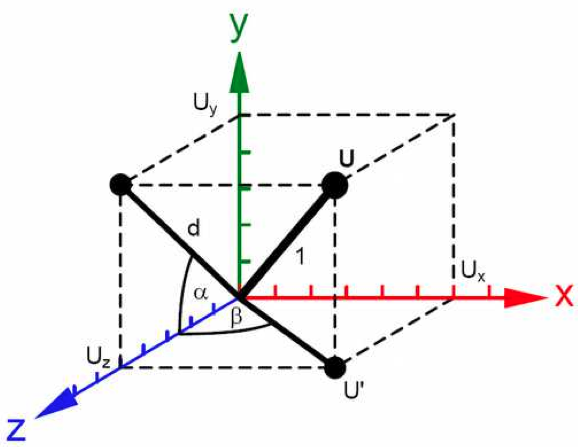
\includegraphics[scale=0.3]{rotation.png}
\end{center}

\newpage
\section{Rasteralgorithmen}
\subsection{Inkrementeller Algorithmus}
\lstinputlisting[style=CStyle,caption=Inkrementeller Algorithmus]{line_increment.c}
\subsection{Bresenham Algorithmus}
\begin{center}
	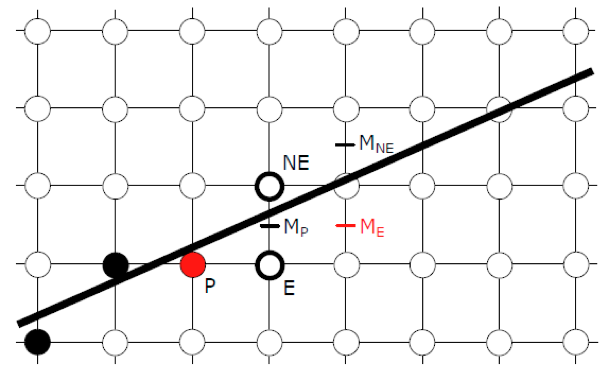
\includegraphics[scale=0.4]{bersenhan.png}
\end{center}
\lstinputlisting[style=CStyle,caption=Bresenham Algorithmus]{bersenhan.c}

\newpage
\section{Perspektive: 3D auf 2D}
\subsection{Kategorien der Projektionen}
Es gibt zwei Arten von Projektionen: perspektivische und parallele. Bei Parallelprojektionen ist der Blickpunkt unendlich weit entfernt, wodurch sich parallele Projektionsstrahlen ergeben. Im Gegensatz dazu führen die Projektionsstrahlen bei Zentralprojektionen ins Zentrum, in den Blickpunkt.
\begin{center}
	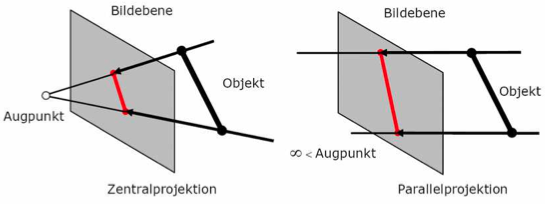
\includegraphics[scale=0.4]{projektionen.png}
\end{center}
\subsection{Parallelprojektion}
Bei Parallelprojektionen sind die Projektionsstrahlen parallel zueinander. Sie können gegen die Projektionsebene schief oder senkrecht (orthogonal) stehen. Parallelprojektionen werden vor allem in technischen Zeichnungen verwendet, um die Tiefeninformationen ablesbar zu halten. Im Gegensatz zur Perspektive sind weiter entfernte Objekte nicht kleiner als nahe Objekte. 
\begin{center}
	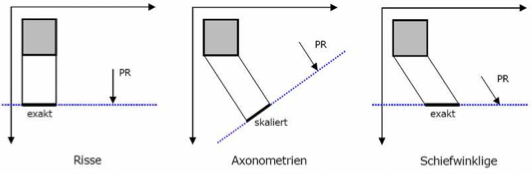
\includegraphics[scale=0.4]{parallelprojektion.png}
\end{center}
\subsection{Zentralprojektion}
Durch die Zusammenführung der Projektionsstrahlen im Projektionszentrum entsteht eine optische Tiefenwirkung. Das Sichtvolumen (Englisch für View Frustum) entspricht bei der perspektivischen Projektion einem Pyramidenstumpf. Es wird wie das orthogonale Sichtvolumen durch die Parameter t=top, l=left, r=right, b=bottom, n=near und f=far definiert:
\begin{center}
	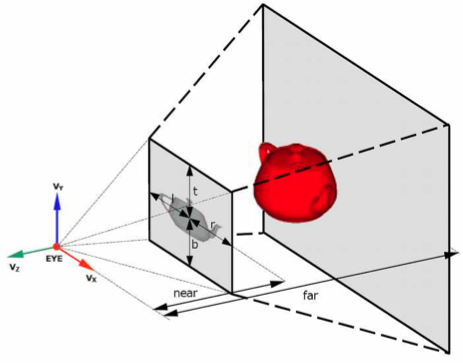
\includegraphics[scale=0.4]{zentralprojektion.png}
\end{center}
\subsection{Projektionstransformation}
Wir können View-Koordinaten nicht auf die Near-Clipping Plane projizieren. Ein zusätzlicher Schritt, die perspektivische Normalisierung ist notwendig. Die perspektivische Transformation kann in vier Schritte zerlegen werden:
\begin{enumerate}
	\item Scherung H in eine orthogonale Sichtpyramide
	\item Skalierung S in ein kanonisches Sichtvolumen
	\item Projektive Transformation N in einen Sichtwürfel 
	\item Perspektivische Division
\end{enumerate}
\subsubsection{Schritt 1: Scherung H in eine orthogonale Sichtpyramide}
Ist die Blickrichtung (Mittellinie der Pyramide) nicht parallel zur negativen z-Achse und somit nicht rechtwinklig zur Projektionsfläche, so muss sie zuerst mit einer Scherung H mit der z-Achse in Übereinstimmung gebracht werden.
\begin{center}
	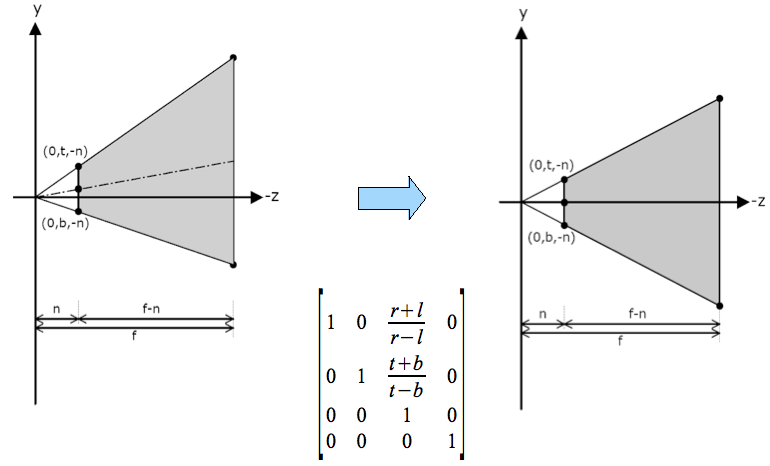
\includegraphics[scale=0.2]{projektionstransformation1.png}
\end{center}
\subsubsection{Skalierung S in ein kanonisches Sichtvolumen}
Stimmt die Blickrichtung mit der negativen z-Achse überein, so wird zur Vereinfachung der perspektivischen Normalisierung im nächsten Schritt mit einer Skalierung S das Sichtvolumen in eine Sichtpyramide transformiert. Die Skalierung betrifft ebenfalls nur die x- und y-Koordinaten.
\begin{center}
	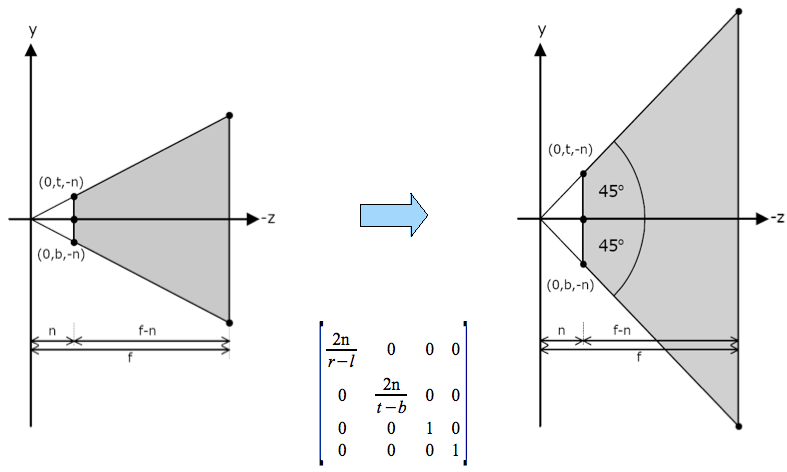
\includegraphics[scale=0.2]{projektionstransformation2.png}
\end{center}
\subsubsection{Projektive Transformation N in einen Sichtwürfel }
\begin{center}
	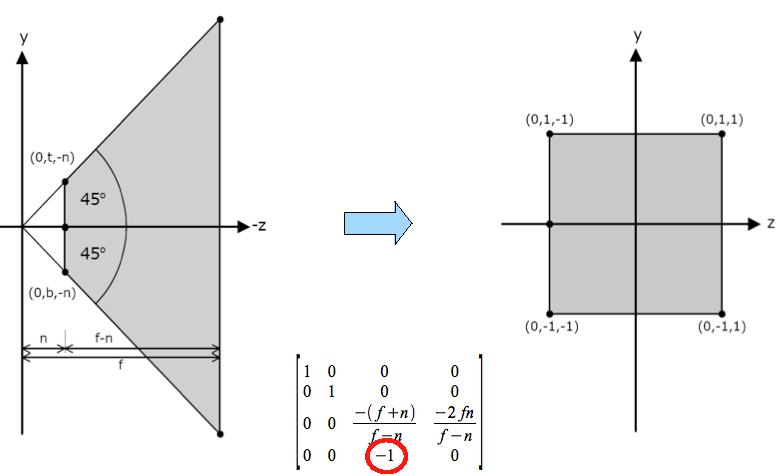
\includegraphics[scale=0.2]{projektionstransformation3.png}
\end{center}
\subsubsection{Perspektivische Division}
Die perspektivische Projektion transformiert die View-Koordinaten in homogene sogenannte Clip-Koordinaten ($C_X$, $C_Y$, $C_Z$, $C_W$). Mit diesen Koordinaten wird in einem nächsten Zwischenschritt das 3D-Clipping durchgeführt. Polygone, die aus der Projektionsebene hinausragen, werden abgeschnitten.
\begin{center}
	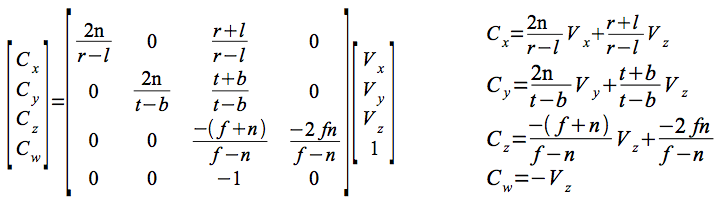
\includegraphics[scale=0.3]{projektionstransformation4_1.png}
\end{center}
Um die gewünschten normalisierten Device-Koordinaten (NDC) ($D_X$, $D_Y$, $D_Z$) zu erhalten, muss nach dem Clipping die Division durch $C_W$ durchgeführt werden. Dieser Schritt wird auch perspektivische Division genannt:
\begin{center}
	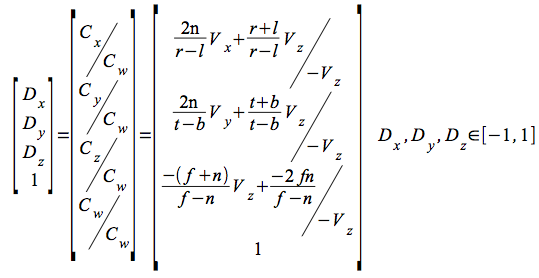
\includegraphics[scale=0.3]{projektionstransformation4_2.png}
\end{center}
\subsection{Viewport-Transformation}
Wir sind mit der Projektionstransformation noch nicht ganz am Ende angelangt. Es fehlt noch die Umrechnung von den normalisierten Device-Koordinaten ($D_X$, $D_Y$, $D_Z$) der virtuellen Projektionsebene zu den Fensterkoordinaten ($S_X$, $S_Y$) und dem Tiefenbufferwert $S_Z$ zwischen $n$ und $f$. Für ein Fenster mit den Fensterkoordinaten von $[x, y]$ unten-links bis $[ww, wh]$ oben-rechts und einem Tiefenbuffer mit Werten zwischen $n$ und $f$ (bei OpenGL normalerweise 0-1) ergäbe sich eine Viewport-Matrix wie folgt:
\begin{equation}
\begin{bmatrix}
S_x \in [x, ww] \\
S_y \in [y, wh] \\
S_z \in [n, f] \\
1
\end{bmatrix} = \begin{bmatrix}
\frac{ww}{2} & 0 & 0 & \frac{x + ww}{2} \\
0 & \frac{wh}{2} & 0 & \frac{y + wh}{2} \\
0 & 0 & \frac{f - n}{2} & \frac{f + n}{2} \\
0 & 0 & 0 & 1
\end{bmatrix}
\end{equation}
\begin{center}
	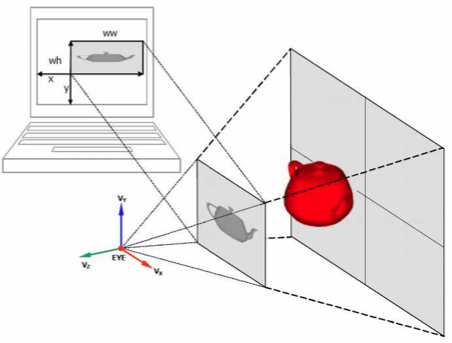
\includegraphics[scale=0.5]{viewport_transformation.png}
\end{center}

\newpage
\section{OpenGL}
\subsection{Was ist OpenGL?}
OpenGL ist ein Software-Interface zur Grafik-Hardware. Das Ziel ist die Echtzeitdarstellung (\textbf{Realtime Rendering}) von \textbf{2D- und 3D-Objekten}. Die Objekte werden durch Raumpunkte (\textbf{Vertizes}) definiert und können durch eine beliebige Transformation auf ein Ausgaberechteck (\textbf{Viewport}) projiziert werden. Die Farbe von jedem Pixel im Ausgabebild kann durch Berechnung und/oder durch Belegung mit Rasterbildern (\textbf{Texture Mapping}) bestimmt werden. \\
OpenGL bietet keine Funktionalität für die Anbindung an ein GUI oder andere betriebssystemabhängige Dienste. Diese werden von den jeweiligen Betriebssystemen bereitgestellt. OpenGL bietet nur primitive geometrische Objekte (Punkte, Linien und Dreiecke) an. \\
OpenGL ist eine Zustandsmaschine (\textbf{State Machine}). Zu jedem Zeitpunkt des Rendering-Prozesses herrscht ein gültiger Zustand. Wird ein Zustand durch ein Ereignis verändert, gilt dieser für alle nachfolgenden Objekte so lange, bis der Zustand wieder verändert wird. Das Setzen der aktuellen Farbe bestimmt z. B. den Zustand der Farbe. Dieser gilt fortan für alle folgenden Objekte, bis der Farbzustand wieder verändert wird. Jede Zustandsvariable hat einen Defaultwert. Der aktuelle Wert eines Zustandes kann mit einer \textbf{glGet*()} Funktion abgefragt werden. Bestimmte Zustände können aktiviert oder deaktiviert werden mit \textbf{glEnable} und \textbf{glDisable}. \\
Das OpenGL API funktioniert nach dem Client/Server Modell, wobei der Client die Applikation und die OpenGL- Implementation der Server ist.
\subsection{Rendering Pipeline}
\begin{center}
	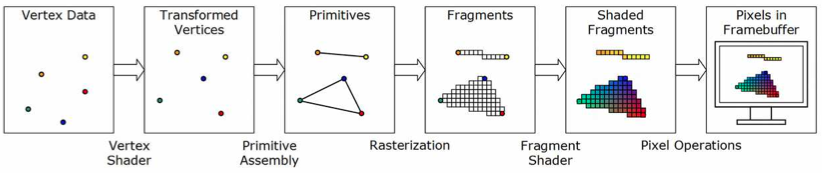
\includegraphics[scale=0.5]{rendering_pipline.png}
	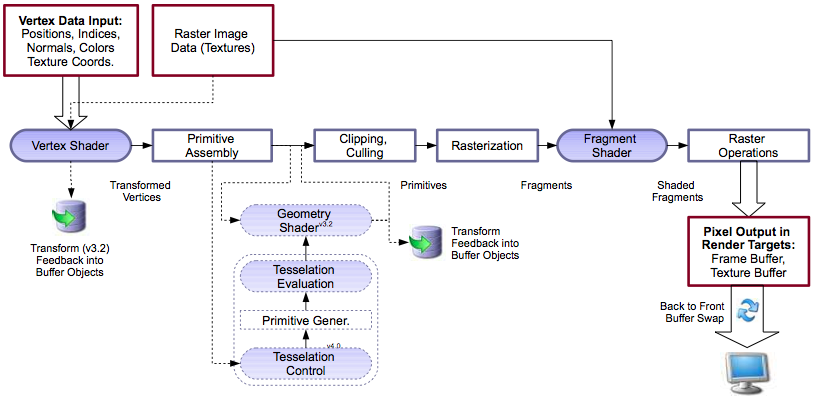
\includegraphics[scale=0.5]{rendering_pipline2.png}
\end{center}
\subsection{Shaders}
Bei der Initialisierung in \textbf{onInit} werden der Quellcode des Vertex Shaders und des Fragment Shaders mit \textbf{loadShader} geladen und mit \textbf{buildShader} und \textbf{buildProgram} kompiliert und zu einem Programm gelinkt.
\lstinputlisting[style=CStyle,caption=Minimaler Vertex Shader]{min.vert}
\lstinputlisting[style=CStyle,caption=Minimaler Fragment Shader]{min.frag}

\newpage
\section{3D-Objekte}
\subsection{OpenGL-Primitive}
\begin{center}
	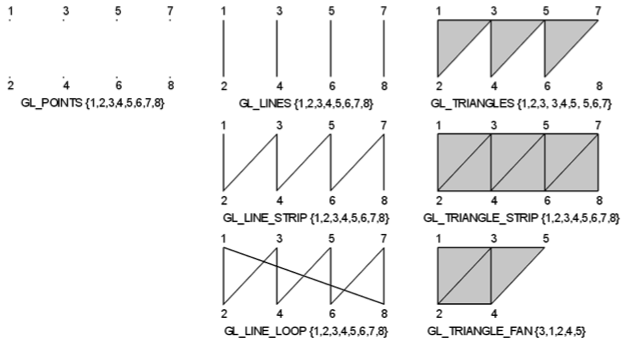
\includegraphics[scale=0.4]{opengl_primitive.png}
\end{center}
\subsection{DrawElements}
Mit dem Zeichnungsbefehl \textbf{glDrawArrays} werden OpenGL-Primitive direkt mit der Vertex-reihenfolge erzeugt. Wird ein Vertex mehrfach in der Geometrie verwendet, so muss er also auch mehrfach im Array vorhanden sein. \\
\\
Mit dem Zeichnungsbefehl \textbf{glDrawElements} werden OpenGL-Primitive anhand eines Index-Arrays gezeichnet. Ein mehrfach vorkommender Vertex muss so nur einmal im Array vorkommen und kann via Index mehrfach referenziert werden. Die Vertexposition verbraucht immerhin 12 Bytes, während ein Index je nach unsigned Datentyp nur 1-4 Bytes belegt.
\lstinputlisting[style=CStyle,caption=Draw Elements]{drawElements.c}

\subsection{Vertex Buffer Object}
Mit jedem Aufruf der Zeichnungsbefehle \textbf{glDrawArrays} und \textbf{glDrawElements} werden die Vertex-Arrays vom Hauptspeicher über den Datenbus auf die Grafikkarte kopiert. Dies ist unumgänglich, wenn sich die Vertexdaten sehr schnell ängern würden. Die allermeisten Objekte bleiben aber über viele Frames, wenn nicht gar für immer gleich. Auch wenn die Objekte sich bewegen, so ändern wir ja nur Transformationsmatrizen und nicht die Struktur der Dreiecksnetze. Es wprde also Sinn machen, wenn wir die Vertex-Arrays im RAM der Grafikkarte speichern könnten und der Kopiervorgang nur einmal durchgeführt werden müsste. Genau diese Möglichkeit bieten uns die Vertex Buffer Objekte.
\lstinputlisting[style=CStyle,caption=VBO erstellen]{buildVBO.c}

\newpage
\section{Shader}
\subsection{Shader Programme kompilieren, linken \& aktivieren}
\begin{center}
	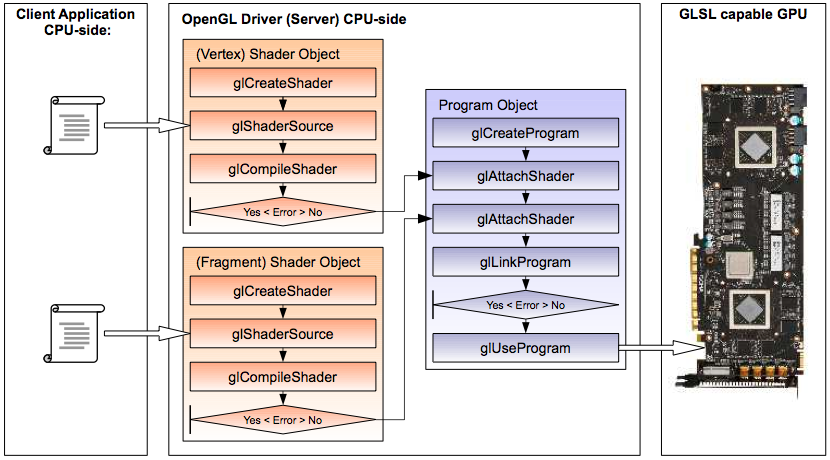
\includegraphics[scale=0.5]{shader.png}
\end{center}
\subsection{einfache Datentypen}
\lstinputlisting[style=CStyle,caption=Datentypen]{glsl_simpleDatatype.c}
\subsection{Typen Qualifizierer}
\subsubsection{const}
\begin{itemize}
	\item Konstanten müssen bei der Deklaration initialisiert werden.
	\item Kann benutzerdefiniert sein.
	\item Kann vordefiniert sein durch GLSL.
\end{itemize}
\subsubsection{attribute}
Mit attribute qualifizierte Variablen dienen als Übergabeparameter der Vertex-Attribute vom Hauptprogramm ans Vertex-Programm. Die Werte können mit jedem Vertex ändern.
\subsubsection{uniform}
Als uniform qualifizierte Variablen dienen als Übergabeparameter vom Hauptprogramm in ein Vertex- oder Fragment-Programm. Deren Werte bleiben für einen ganzen Zeichnungsbefehl konstant.
\subsubsection{varying}
Als varying qualifizierte Variablen dienen als Übergabeparameter vom Vertex- zum Fragment-Programm. Der Wert einer Varying-Variable wird im Vertex-Programm gesetzt und steht dann über das Primitiv interpoliert im Fragment-Programm zur Verfügung.
\begin{center}
	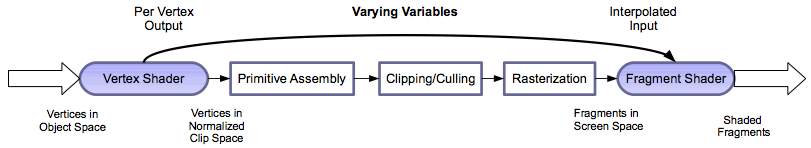
\includegraphics[scale=0.5]{glsl_varying.png}
\end{center}

\newpage
\section{Beleuchtung}
\subsection{Lichtquellen}
\begin{center}
	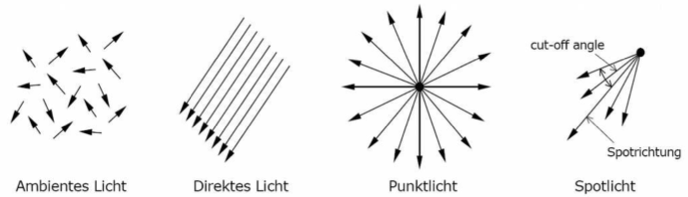
\includegraphics[scale=0.5]{lichtquellen.png}
\end{center}
\subsection{Reflexion}
\subsubsection{Ambiente Reflexion}
$I_a$ bezeichnet darin die konstante, ambiente Lichtintensität und $k_a$ den ambienten Reflexionskoeffizienten (zw. 0 und 1) des reflektierenden Materials. 
\begin{equation}
I_{ambi}=I_a * k_a
\end{equation}
\subsubsection{Diffuse Reflexion}
$I_d$ bezeichnet darin die konstante, diffuse Lichtintensität und $k_d$ den diffusen Reflexionskoeffizienten (zw. 0 und 1). Wenn N und L normalisiert sind, kann der Kosinus durch das Skalarprodukt beider Vektoren ersetzt werden.
\begin{equation}
I_{diff}=I_d * k_d * max( cos(\theta), 0) = I_d * k_d * max(N \bullet L, 0)
\end{equation}
\begin{center}
	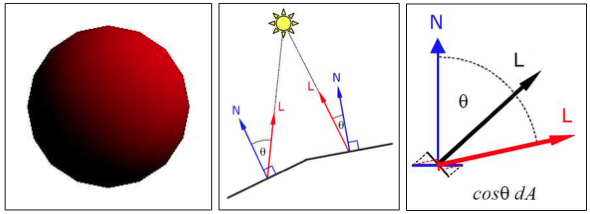
\includegraphics[scale=0.4]{diffuse_reflexion.png}
\end{center}
\subsubsection{Spiegelnde Reflexion}
Die Menge des reflektierten Lichts ist vom Beobachterstandpunkt abhängig bzw. vom Winkel $\alpha$ zwischen dem Beobachtungsvektor E (eye) und dem reflektierten Strahl R, sowie von einer Materialbeschaffenheit $n$ bezüglich der Reflektierbarkeit (Shininess) ab. $I_s$ bezeichnet die konstante, spiegelnde Lichtintensität und $k_s$ den spiegelnden Reflexionskoeffizienten (zw. 0 und 1).
\begin{equation}
I_{spec}=I_s * k_s * max( cos(\alpha), 0)^n = I_s * k_s * max(R \bullet E, 0)^n
\end{equation}
\begin{center}
	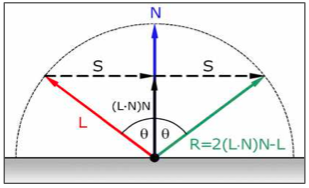
\includegraphics[scale=0.4]{reflektierender_strahl.png}
	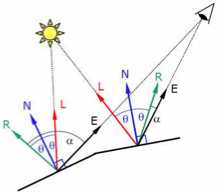
\includegraphics[scale=0.4]{spiegelnde_reflexion.png}
\end{center}
\subsubsection{Lichtabnahme (Attenuierung)}
Bevor wir alles zusammenstellen können, müssen wir noch die Energieabnahme des Lichts (Lichtabnahme) in Abhängigkeit der Distanz berücksichtigen. Darin sind $c_1$, $c_2$ und $c_3$ Konstanten für die konstante, die lineare und die quadratische Lichtabnahme in Abhängigkeit der Distanz $d$. Diese Lichtabnahme wirkt nur auf die diffuse und die spiegelnde Reflexion.
\begin{equation}
f_{att}=min(\frac{1}{c_1 + c_2 * d + c_3 * d^2}, 1)
\end{equation}
\subsection{Beleuchtungsmodell nach Phong}
\begin{equation}
	I_{Phong}=I_{amb} + \sum_{i=0}^{lights-1} f_{att} * (I_{diff} + I_{spec})
\end{equation}
\subsection{Erweiterungen im alten OpenGL Beleuchtungsmodell}
\begin{equation}
	I_{OpenGL}=k_e + I_{aglobal} * k_{aglobal} + \sum_{i=0}^{lights-1} f_{att} *  S_{spott} * (I_{ambi} + I_{diff} + I_{spec})
\end{equation}
\begin{description}
	\item[Emittierende Farbintensität] $k_e$ für selbststrahlende Objekte
	\item[Globale ambiente Hintergrundintensität] $I_{aglobal}$ unabhängig von einer Lichtquelle
	\item[Spotlichteffekt] $S_{spot}$ bewirkt die Begrenzung des Spotlichts und eine Lichtabnahme innerhalb des Lichtkegels von der Spotachse zum Kegelrand bewirkt. Der Wert von Sspoteffect ist:
	\begin{itemize}
		\item 1, wenn das Licht kein Spotlicht ist (Cut-Off Winkel=180).
		\item 0, wenn das Licht ein Spotlicht ist, der Vertex aber ausserhalb des Spotkegels ist.		
		\item $max(L \bullet S , 0)^{spotexp}$ , wobei L der Vektor von der Vertexposition zum Licht ist und S die Spotrichtung und spotexp ein Exponent zwischen 0 und 128. Standardwert ist 0.
		\item Ein zunehmender Exponent bewirkt eine Abnahme des Lichtes zum Kegelrand.
	\end{itemize}
\end{description}
\subsection{Blinn's Halbvektor}
Jim Blinn steuerte eine vereinfachte Berechnung des spekulären Anteils bei, indem er den Winkel zwischen der Normalen N und einem Halbvektor H berechnet. H ist der normalisierte Halbvektor zwischen der Blickrichtung E und der Lichtrichtung L.
\begin{equation}
I_{specBlinn}=I_s * k_s * max(N \bullet H ,0)^n
\end{equation}
\begin{equation}
(R \bullet E)^n \approx (N \bullet H)^{4n}
\end{equation}
\subsection{Schattierung}
\subsubsection{Berechnung pro Dreieck: Flat Shading}
Im alten OpenGL war es möglich die Beleuchtungsrechnung auf den letzten Vertex eines Polygons zu beschränken. Dies bewirkte eine flache Schattierung und war die einfachste und schnellste Beleuchtung.
\subsubsection{Berechnung pro Vertex: Gouraud Shading}
Im alten OpenGL wurde die Blinn'sche Version des Phong Modells pro Vertex gerechnet und die Farbwerte dann über das Polygon interpoliert. Dabei werden die Farbwerte zwischen den Eckpunkten eines Polygons linear interpoliert. Der Scanline Algorithmus wird ist in folgende Schritte gegliedert:
\begin{enumerate}
	\item An allen Ecken eines Dreiecks müssen die Normalen definiert sein, die aus den Flächennormalen der jeweiligen Nachbardreiecke gemittelt wurden.
	\item Die Farbwerte an den Ecken gemäss Beleuchtungsmodell bestimmen.
	\item Pixelzeile für Pixelzeile werden die Kantenwerte linear interpoliert.
	\item Pixelintensitäten berechnen durch Interpolation zwischen den Werten.
\end{enumerate}
\textbf{Nachteile}:
\begin{itemize}
	\item  Ungenaue Glanzlichter
	\item Keine Lichtkegel
	\item Keine perspektivische Verzerrungen
	\item Abhängigkeit von der Orientierung
	\item Nicht repräsentative Knotennormalen
\end{itemize}
\begin{center}
	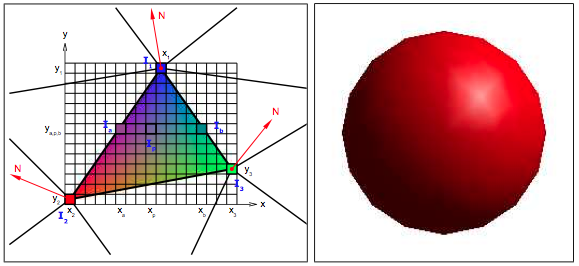
\includegraphics[scale=0.4]{gouraud_shading.png}
\end{center}
\subsubsection{Berechnung pro Pixel: Phong Shading}
Es liegt auf der Hand, dass die Phong Shading wesentlich aufwendiger ist, wenn die gesamte Rechnung pro Pixel anstatt nur pro Vertex gemacht werde muss. Zusätzlich muss ja vorgängig für jedes Pixel eine interpolierte Normale und Pixelposition berechnet werden. \\
\\
\textbf{Nachteile}:
\begin{itemize}
	\item Polygonale Silhouetten
	\item Spotlichtgrenzen nicht auf Kugeloberflächen
\end{itemize}
\begin{center}
	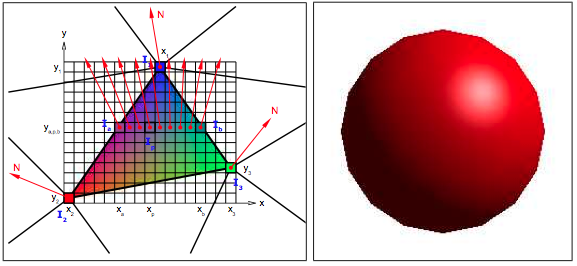
\includegraphics[scale=0.4]{phong_shading.png}
\end{center}

\newpage
\section{Texture Mapping}
\subsection{verschiedene Texturen}
\begin{center}
	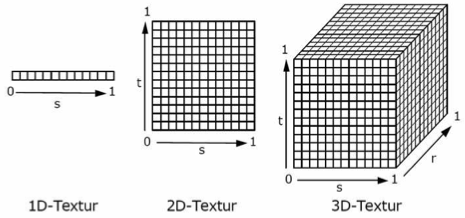
\includegraphics[scale=0.4]{texturen.png}
\end{center}
\subsection{Textur Abbildung}
\begin{center}
	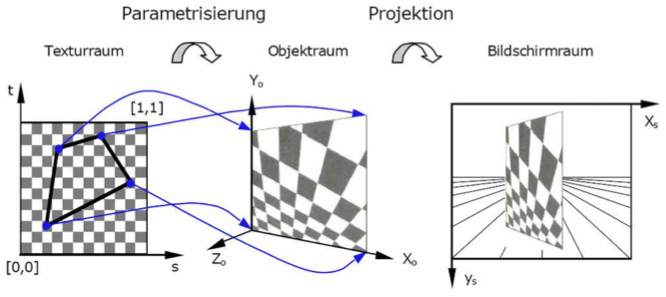
\includegraphics[scale=0.4]{textur_abbildung.png}
\end{center}
\subsection{Texturfilterung}
\begin{center}
	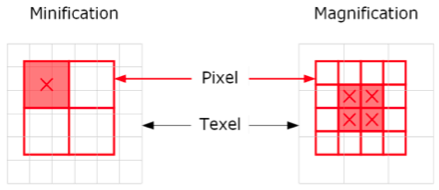
\includegraphics[scale=0.4]{texture_sampling.png}
\end{center}
\subsubsection{Point Sampling}
Wird keine Filterung angewendet, so wird nach der Point Sampling oder Nearest Neighbour Methode gearbeitet, bei der das dem Pixelzentrum (Kreuz) am nächsten liegende Texel verwendet wird. Dies ist also im Prinzip nur ein Abschneiden der Nachkommastellen.
\subsubsection{Bilineare Filterung}
Bei der bilinearen Filterung werden die benachbarten Texel mit berücksichtigt. Da in X- und Y-Richtungen interpoliert wird, nennt man diesen Filter bi-linear.
\begin{center}
	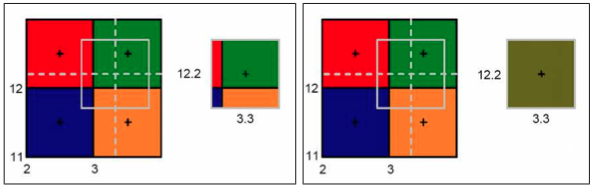
\includegraphics[scale=0.4]{bilineare_filterung.png}
\end{center}
\subsubsection{MIP-Mapping}
Die Idee dahinter ist, eine Textur bereits vor der Anwendung mit mehreren Verkleinerungen anzulegen, um diese je nach Distanz zum Betrachter einzusetzen.
\begin{center}
	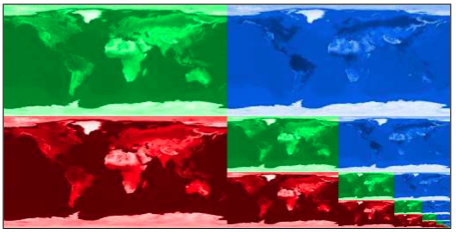
\includegraphics[scale=0.4]{mip-mapping.png}
\end{center}
\subsubsection{Trilineare Filterung}
Der Übergang von einem MIP-Level zum nächsten fällt besonders bei grossen Flächen mit gleicher Textur auf. Die verschieden aufgelösten MIP-Level bilden dabei eine scharfe Kante. Beim trilinearen Filtern werden nun zuerst die entsprechenden Texel der zwei MIP- Levels bilinear gefiltert und diese dann noch einmal linear (eben tri) zwischen den beiden MIP-Levels.
\begin{center}
	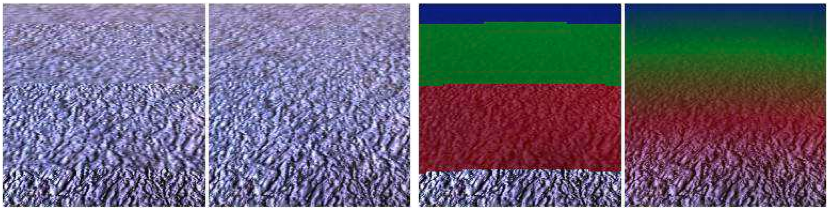
\includegraphics[scale=0.4]{trilineare_filtering.png}
\end{center}
\subsubsection{Anisotropische Filterung}
Die trilineare Filterung hat nur noch einen Mangel. Die perspektivische Verzerrung wird zwar bei der Bestimmung der Texel-Position berücksichtigt, bei der bilinearen Interpolation fällt sie aber unter den Tisch. Man müsste Texturen, auf die man sehr schräg sieht, mit anderen Verfahren filtern als jene, auf die man senkrecht sieht. Da für beste Qualität nicht mehr isotrop, also gleichmässig gefiltert werden kann, muss das ungleichmässig (sprich anisotrop) getan werden. Beim bilinearen Filtern werden bekanntlich nur 4 Texel gemischt. Für den trilinearen Filter sind 2 bilinear gefilterte Texel.
\begin{center}
	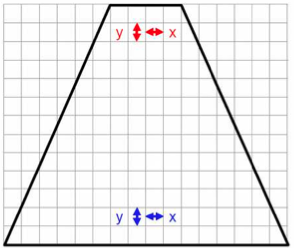
\includegraphics[scale=0.4]{anisotropische_filterung.png}
\end{center}

\subsection{Bump Mapping}
\begin{center}
	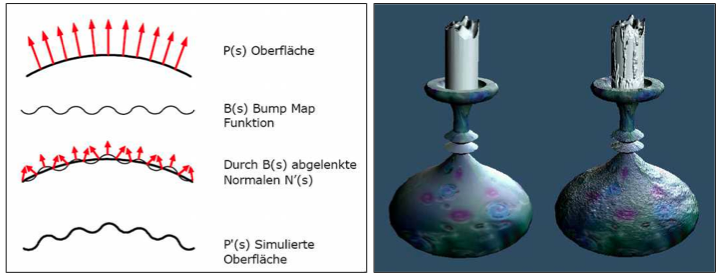
\includegraphics[scale=0.3]{bump_mapping.png}
\end{center}
\subsubsection{Heightfield Bump Mapping}
Die Normale wird durch einen Vektor D abgelenkt, indem er zur Normalen hinzuaddiert wird. Der Ablenkungsvektor D berechnet sich aus den Tangentialvektoren T und B (Binormale) sowie aus der partiellen Ableitung d (= Grauwertsteigung) bei der Texturkoordinate s,t in der Bumpmap.
\begin{center}
	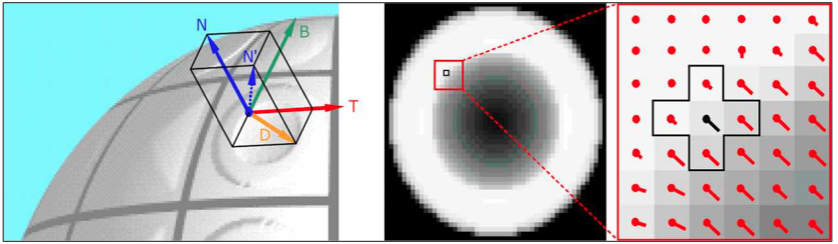
\includegraphics[scale=0.4]{heightfield_bump_mapping.png}
\end{center}
\subsubsection{Normalmap Bump Mapping}
Eine Verbesserung hinsichtlich der Performanz ist das sogenannte Normalmap Bump Mapping. Dabei wird die bereits abgelenkte Normale im Tangentenraum in einem RGB- Bild abgespeichert. Die Koordinatenkomponenten x, y und z entsprechen den Farbkomponenten r, g und b.
\begin{center}
	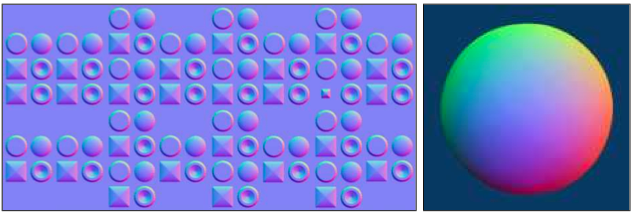
\includegraphics[scale=0.4]{normalmap_bump_mapping.png}
\end{center}
\subsubsection{Parallax Mapping}
Die Grundidee besteht darin die Texturkoordinaten (im Bild neben an nur die T-Komponente) so zu dehnen, dass wir sie den Höhen entsprechend richtig sehen. Für den Punkt P im Bild neben an würden wir ohne Parallax Mapping das Texel bei T erhalten, obwohl wir eigentlich die Farbe bei $T_I$(deal) sehen sollten. Um diese Berechnung zu vereinfachen, beschränkt man den Versatz um die Höhe H entlang des Augvektors E.
\begin{center}
	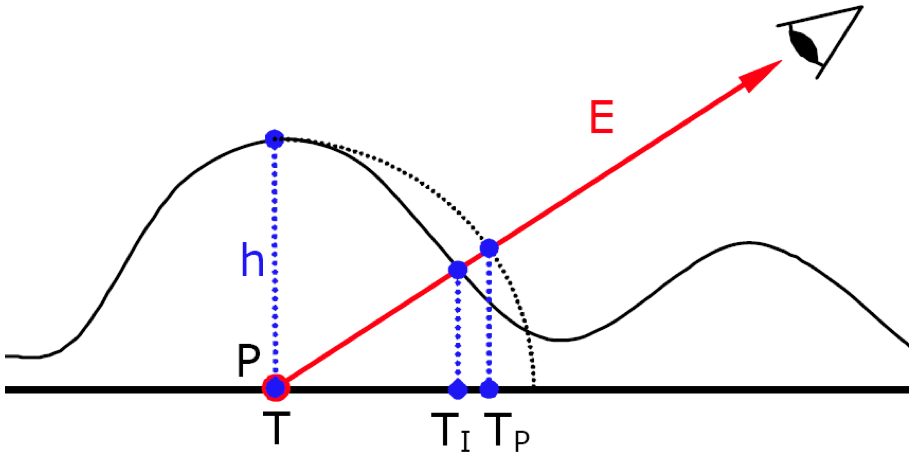
\includegraphics[scale=0.2]{parallax_mapping.png}
\end{center}

\subsection{Texture Mapping in OpenGL}
\begin{enumerate}
	\item Texturnamenanlegen.
	\item Textur binden(aktivieren). 
	\item Texturparameter setzen. 
	\item Texturdaten übergeben
	\item Mipmap-Level generieren.
\end{enumerate}

\newpage
\section{Frustum Culling}
\subsection{Ziel}
Ziel ist es, nur Objekte durch die Pipeline zu schicken, die sichtbar sind:
\begin{center}
	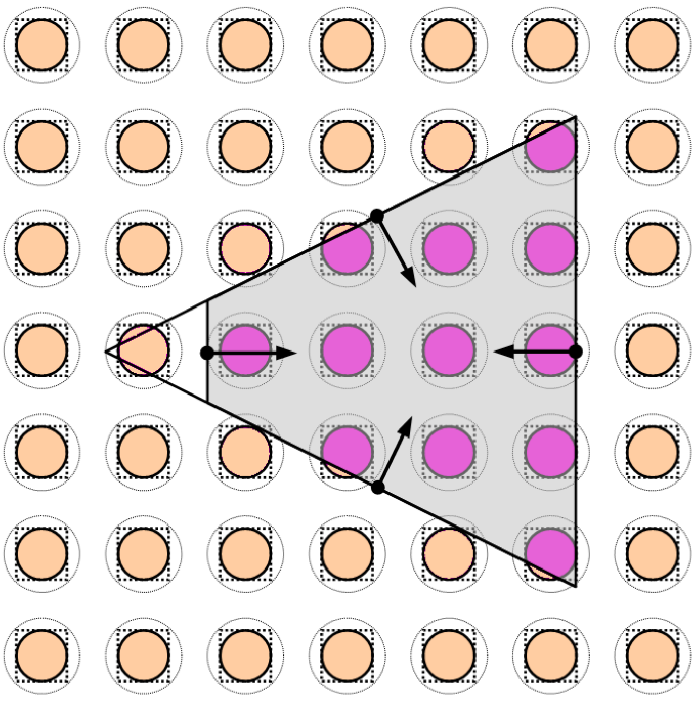
\includegraphics[scale=0.2]{frustum_culling.png}
\end{center}
\subsection{Hüllvolumen}
Die Wahl des Hüllvolumens hängt von folgenden Kriterien ab:
\begin{itemize}
	\item Passgenauigkeit des Hüllvolumens
	\item Kosten des Hüllvolumenschnitttests. 
	\item Erstellungskosten des Hüllvolumens.
\end{itemize}
\subsection{AABB (axis-aligned bounding box)}
Die AABB für eine bestimmte Punktmenge ist die minimale bounding box mit der Einschränkung, dass die Kanten der Box parallel zu den (kartesischen) Koordinatenachsen sind. Es ist lediglich das kartesische Produkt der $N$ Intervalle, von denen jeder durch den minimalen und maximalen Wert der entsprechenden Koordinaten, für die Punkte in $S$, definiert sind.\\
\begin{center}
	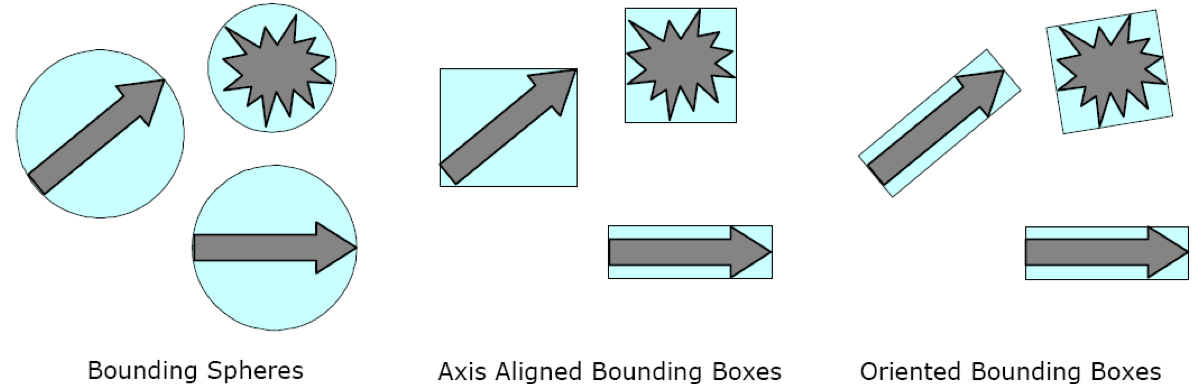
\includegraphics[scale=0.3]{huellvolumen.png}
\end{center}
Aufwand für die Berechnung des Hüllvolumens für ein Objekt, dass sich bewegt muss unter Umständen von Frame zu Frame neu berechnet werden. Wissen wir nichts über die Struktur des zu umhüllenden Objekts, so ist die AABB mit Abstand am einfachsten zu berechnen. Wir suchen einfach das Minimum und das Maximum aller Koordinatenkomponenten.\\
Die kleinste umgebende Kugel zu finden ist dagegen viel aufwendiger. Der Aufwand lohnt sich meistens nicht, weshalb man eine Methode verwendet, die eine um ca. 5\% grössere Kugel berechnen kann.\\
Um den kleinsten Kubus um n Punkte zu berechnen, verwendet man eine statistische Methode, genannt Principal Component Analysis. Man findet dabei die primären Achsen, entlang deren die Koordinaten am meisten variieren.


\newpage
\section{Alpha Blending}
\subsection{Einleitung}
\begin{itemize}
	\item Beim Alpha Blending wird eine neue Farbe mit der bestehenden vermischt.
	\item Der Alpha Wert ist der Dekungsgrad.
	\item Der Alpha Wert der Farbe ist der 4. Parameter bei den Farbangaben RGB\Bold{A}.
\end{itemize}
\subsection{Berechnung}
\begin{center}
	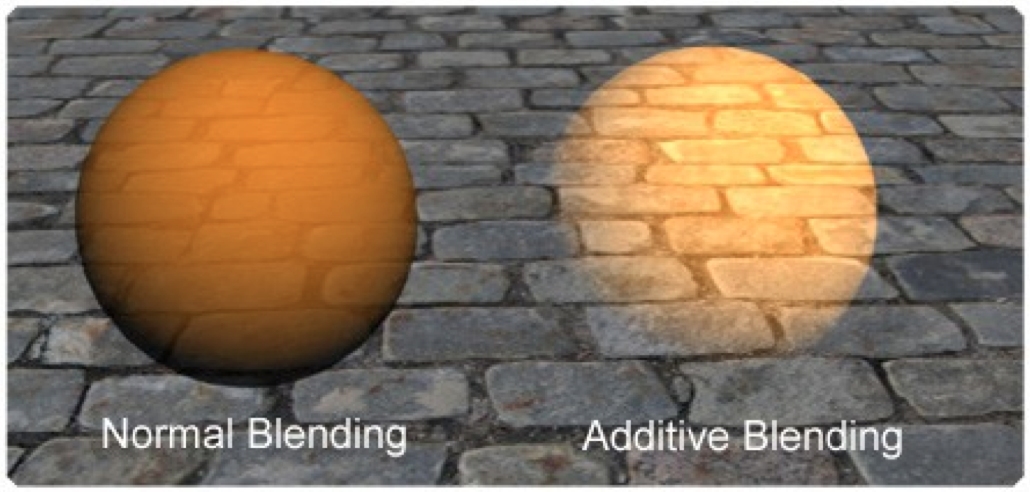
\includegraphics[scale=0.2]{additive_blending.png}
\end{center}
Normal Blending:
\begin{equation}
	Color = C \cdot \alpha + C_{bg} \cdot (1 - \alpha)
\end{equation}
Additive Blending:
\begin{equation}
	Color = C \cdot \alpha + C_{bg}
\end{equation}

\subsection{Zeichnungsreihenfolge}
Zeichnungsreihenfolge ist entscheidend:
\begin{enumerate}
	\item Alle opaqen (=nicht-transparente) Objekte
	\item Alle transparenten Objekte
\end{enumerate}
In diesem Beispiel wurde zuerst die blaue Box, dann die rote Box und schlussendlich die grüne Box gezeichnet. Auf der rechten Seite wurde die selbe Reihenfolge benutzt aber die Ansicht wurde gedreht.
\begin{center}
	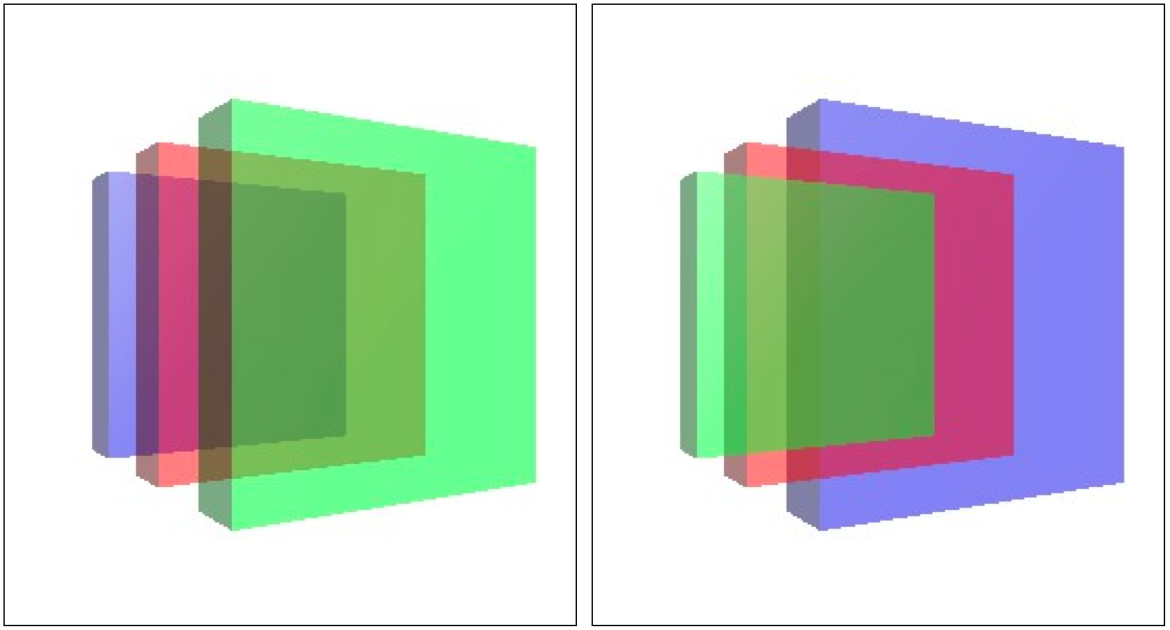
\includegraphics[scale=0.2]{alphablending_order.png}
\end{center}
Eine korrekte Transparenz können wir nur erreichen, wenn wir zuerst undurchsichtige (Englisch: opaque) Objekte mit eingeschaltetem Z-Buffer und dann die transparenten Objekte, von hinten nach vorne sortiert, mit ausgeschaltetem Z-Buffer-Test zeichnen.


\newpage
\section{Deferred Shading}
Methode um in dreidimensionalen Szenen die Geometrieverarbeitung von der Lichtberechnung zu trennen. So sind mehrere hundert dynamische Lichter in geometrisch komplexen Szenen möglich
\subsection{Prinzip}
In klassischen Rendermethoden wird anhand von Tiefe (depth), Ausrichtung (normals) und Farbe (albedo) eines Eckpunktes und Farbe, Intensität und Einfallswinkel einer Lichtquelle der finale Farbwert für den jeweiligen Eckpunkt ermittelt. Für jede Lichtquelle muss so jeder Eckpunkt zur Berechnung herangezogen werden. \\
Beim Deferred Shading werden nun Tiefenwert, Ausrichtung und Farbe eines jeden Pixels in jeweils eine Textur in Bildschirmgröße gespeichert. Dies wird durch sogenannte Multiple Render Targets ermöglicht, wobei in jedem Rendervorgang in verschiedene Framebufferobjekte (die Texturen) gleichzeitig geschrieben werden kann. Statt dass nun jeder Eckpunkt mit den Lichtquellen verrechnet werden muss, muss nur noch jedes Pixel (in dem alle benötigten Werte – depth, normals und albedo – vorhanden sind) bei der Berechnung berücksichtigt werden. \\
Die Berechnung selbst erfolgt durch klassische Beleuchtungsmodelle, wie zum Beispiel nach Phong. Dabei kann zusätzlich noch Glanzlicht mit einbezogen werden. Technisch geschieht das im Pixel- bzw. Fragment-Shader am Ende der Grafikpipeline.
\begin{center}
	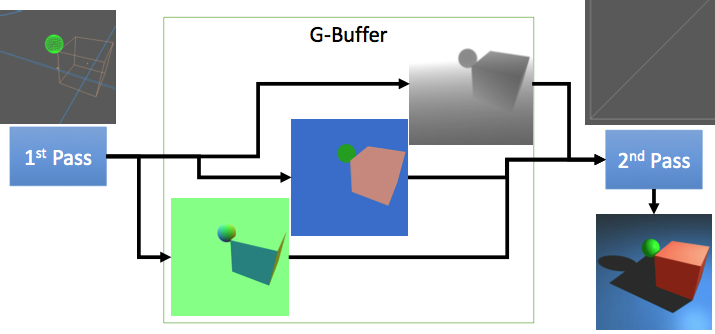
\includegraphics[scale=0.4]{deferred-rendering.png}
\end{center}

\subsection{Vorteile}
\begin{itemize}
	\item Independent of scene complexity \& dynamics.
	\item Fully in hardware.
	\item Well suited for deferred renderers (as normal map is typically available).
\end{itemize}
\subsection{Nachteile}
\begin{itemize}
	\item Noise removal requires extra blur stage.
	\item Limited range of sample sphere makes approach relatively local and view dependent.
\end{itemize}
\subsection{OpenGL}
\subsubsection{Framebuffer objects}
\begin{itemize}
	\item FBOs encapsulate a framebuffer that can be used for off- screen rendering.
	\item Each FBO has a given dimension, and a number of attachments (n color buffers, depth buffer, and stencil buffer).
	\item Attached buffers are either textures or renderbuffers. 
	\item FBOs can be enabled for writing and reading.
\end{itemize}
\subsubsection{FBO relevant API}
\begin{itemize}
	\item glGenFramebuffer, glDeleteFramebuffers
	\item glBindFramebuffer - Bind for reading or writing
	\item glClearBuffer
	\item glFramebufferTexture2D - Attach texture to FBO
	\item glCheckFramebufferStatus -  Important: Check if FBO is correctly set up
\end{itemize}

\newpage
\section{Shadow Rendering}
\subsection{Shadow Maps}
Beim Shadow Mapping werden Schatten generiert, indem getestet wird, ob ein Pixel von einer Lichtquelle aus sichtbar ist. Dabei wird zunächst die sogenannte Shadow Map erzeugt. Diese ist eine aus Sicht der Lichtquelle erzeugte Tiefenkarte. Diese enthält Informationen über den geringsten Abstand von Objekten einer Szene zur Lichtquelle (Z-Buffer). Durch den Vergleich des Abstandes des zu rendernden Objektes zur Lichtquelle und dem entsprechenden Punkt in der Shadow Map kann der Schattenwurf berechnet werden.
\subsection{Cascade Shadow Maps}
\begin{center}
	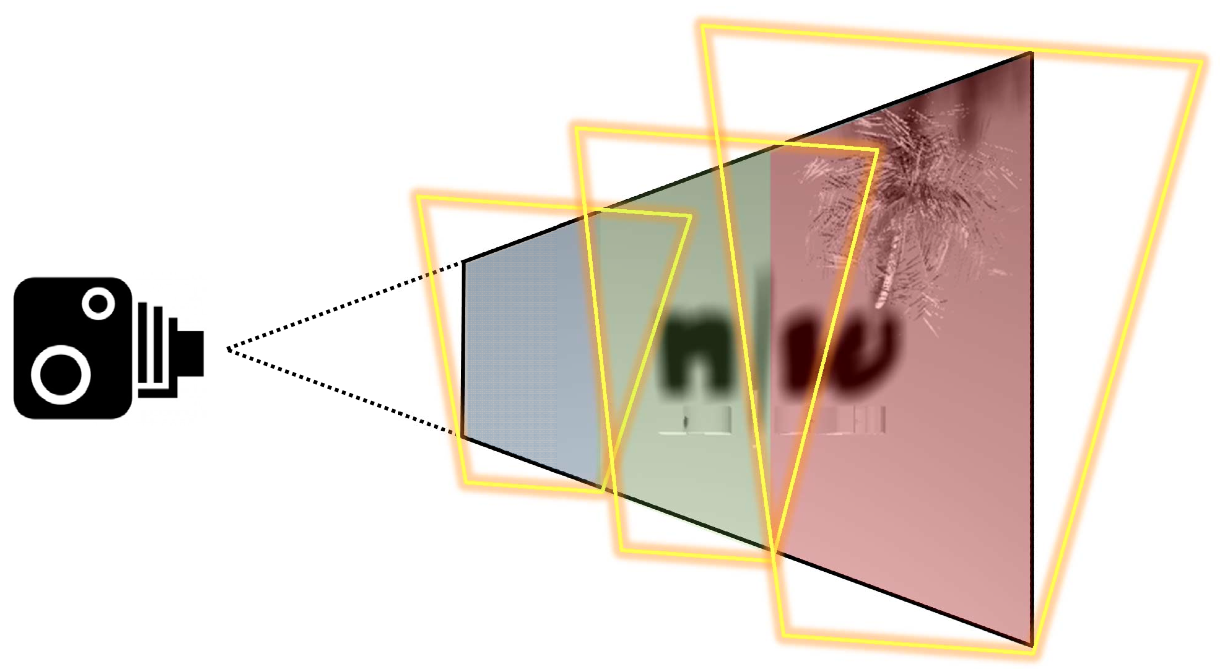
\includegraphics[scale=0.15]{cascade_shadow_maps.png}
\end{center}
\subsection{Vergleich}
\begin{center}
	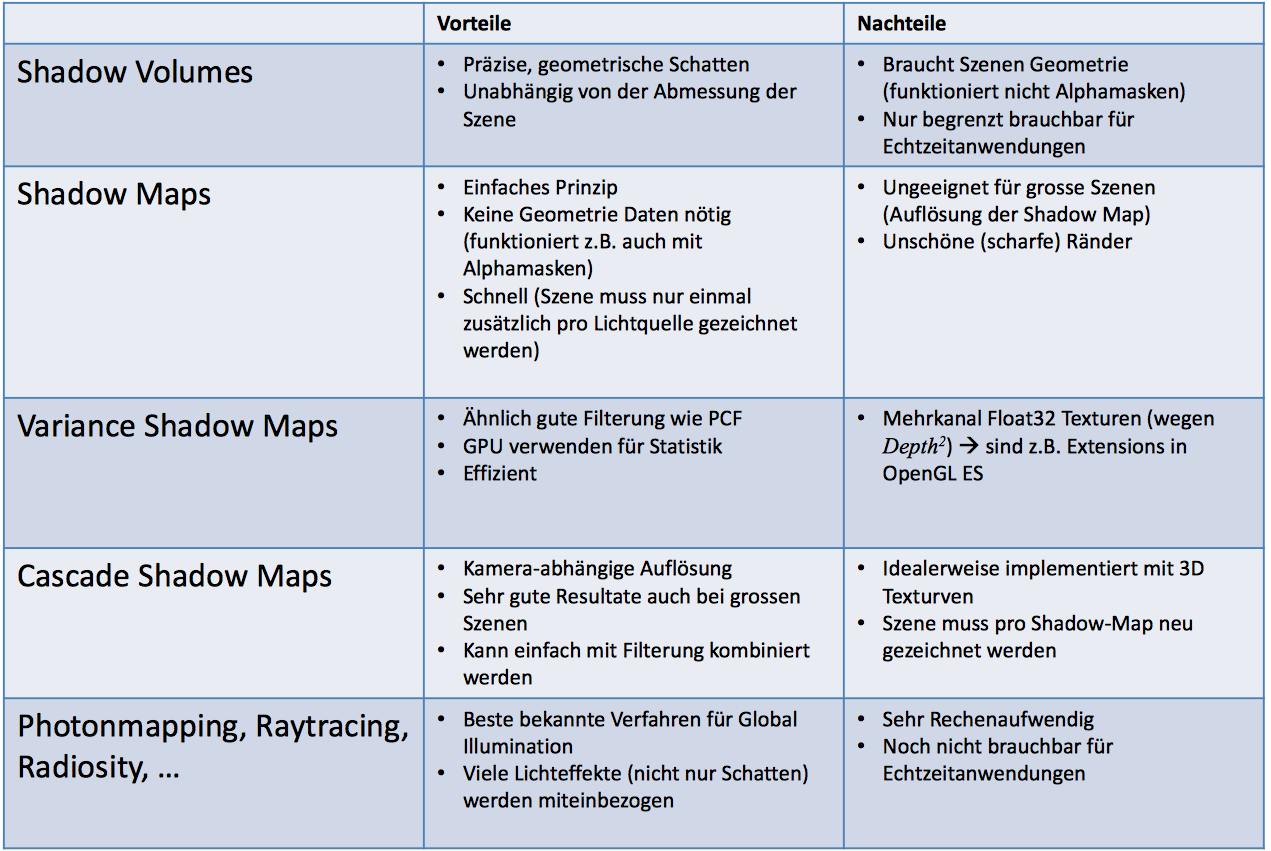
\includegraphics[scale=0.35]{shadow_rendering.png}
\end{center}

\newpage
\section{Stereoprojektion}
\subsection{Raumwahrnehmung}
\subsubsection{Teifenunschärfe}
Bis zu einer Entfernung von 10m kann das Gehirn aus der Fokussierung eine Teifeninformation gewinnen. Je näher der fokusierete Gegenstand ist, umso präziser muss die Fokussierung arbeiten und umso grösser ist die Tiefenunschärfe. Beim Tilt-Shift-Effekt wird eine räumliche weite Szenerie durch künstliche Unschärffe so dargestellt, als ob si im Massstab einer Modelleisenbahn wäre.
\subsubsection{Abnehmende Grösse}
Durch die Zentralperspektive erscheinen weiter entfernte Gegenstände kleiner.
\subsubsection{Zunehmender Dunst}
Mit zunehmender Distanz nimmt der Dunst zu und die Silhouetten von Bergketten werden heller. Dieser Effekt lässt sich mit OpenGL leicht imitieren, indem man jedem Pixel mit zunehmender Distanz eine Dunstfarbe hinzuaddiert.
\subsubsection{Schettenbildung}
Wir sind uns gewohnt, dass das Licht von oben kommt. Ist dem nicht so, so haben wir Mühe die Dreidimensionalität  zu verstehen.
\subsubsection{Bewegungsparallaxe}
Einfache Games und Trickfilme verwenden oft den Trick der Bewegungsparallaxe, bei der sich nahe Objekte schneller bewegen als Objekte weiter hinten. Damit erreicht man einen Tiefeneffekt, obwohl es eine reine 2D-Animation ist.
\subsection{Stereobildwiedergabe}
\subsubsection{Projektion nebeneinander}
Techniken wie das Spiegelstereoskop, Stereoskope und Stereobrillen führen den beiden Augen durch Spiegel, spezielle Linsen oder Brillen getrennt das jeweilige Bild zu. Sie haben den Vorteil, dass sie eine hundertprozentige Bildtrennung gewährleisten aber auch den Nachteil, dass sie auf einen Betrachter beschränkt sind.
\subsubsection{Projektionen übereinander}
\begin{description}
	\item[Trennung durch Farbfilter] \hfill \\
		Das älteste Verfahren zu Auftrennung von zwei übereinander gelagerten Bildern durch Farbfilter ist nur ein wenig jünger als die Fotografie selbst. Beil solchen Anaglyphen-Bildern wird das Bild für das linke Auge meist in Rot und das Bild für das rechte Auge in Cyan dargestellt. Mit einer Brille, die vor dem linken Auge einen Rotfilter und vor dem rechten Auge einen Cyan-Filter hat, werden die Teilbilder für die entsprechenden Augen herausgefiltert. \\
		Es gibt verschiedene Typen:
		\begin{description}
			\item[Echte Anaglyphen] \hfill \\
				Hier findet eine Graukonversion auf dem Rot- und Blau-Kanal statt. Dies entspricht den ursprünglichen Anaglyphen und ergibt ein relativ dunkles Bild und es gibt praktisch kein Ghosting (Überblenden), da die Kanäle nicht aneinandergrenzen.
			\item[Graue Anaglyphen] \hfill \\
				Diese echten Rot-Cyan-Anaglyphen ergeben ebenfalls ein Graustuffenbild. Die Helligkeit ist dabei korrekt aber durch die benachbarten Rot- und Grün-Kanäle entsteht mehr Ghosting
			\item[Farbige Anaglyphen] \hfill \\
				Bei diesen werden die Farbkanäle nicht skaliert. So kann ein Grossteil der Farben wiedergegeben werden. Allerdings ist das Ghosting sehr stark.
			\item[Halbfarbige Anaglyphen] \hfill \\
				Setzt man den Rotkanal als Graustufe zusammen, vermindert sich das sich das Ghosting aber auch die Farbwiedergabe.
			\item[Optimierte Anaglyphen] \hfill \\
				Gibt man den Rotkanal ganz auf und gewichtet Grün und Blau stärker, wird das Bild aufgehellt und das Ghosting ist fast ganz eliminiert.
			\item[ColorCode3D Anaglyphen] \hfill \\
				Damit kann eine fast vollständige Farbwiedergabe gewährleistet werden. Das Farbspektrum wird für das linke Auge im Rot-Grün-Spektrum wiedergegeben und die Helligkeit auf dem rechten Auge im Blauspektrum. Ein weiterer Vorteil ist, dass auch die Betrachtung ohne die gelb-blaue Color-Code-Brille fast ungestört möglich ist.
		\end{description}
	\item[Trennung durch Polarisationsfilter] \hfill
		\begin{description}
			\item[Lineare Polarisationsfilter] \hfill \\
				Diese lassen nur Licht einer bestimmten Polarisationsrichtung passieren. Damit die Polarisationsrichtung erhalten bleibt, muss eine versilberte Leinwand verwendet werden un der Betrachter muss den Kopf waagrecht halten, um eine Vermischung zu vermeiden. \\
				Sie Werden auch in Sonnenbrillen eingesetzt, um den Himmel abzudunkeln oder um Spiegelungen auf Festerschreiben herauszufiltern.
			\item[Zirkuläre Polarisationsfilter] \hfill \\
				Diese filtern das Licht zweistuffig. Zuerst wird es linear gefiltert und dann wird es mit einem Lambda/4-Filter in Drehung versetzt. Links und rechts unterscheiden sich durch umgekehrte Drehrichtungen.
		\end{description}
	\item[Trennung durch Interferenzfilter] \hfill \\
		Diese fitlern enge Frequenzbänder aus dem Gesamtpspektrum heraus. Jedes Auge erhält dabei ein unterschiedliches Rot-,Grün- und Blau-Frequenzband. Die Farbtrennung dabei ist praktisch 100\% und es braucht zudem keine Silberleinwand.
	\item[Zeitliche Trennung durch Shutter-Brillen] \hfill \\
		Das linke und rechte Bild wird nacheinander projiziert. Abwechlungsweise blockieren die Brillengläser die Sicht eines Bildes. Durch eine schnelle Abwechslung entsteht  ein konstanter Bildeindruck. 
\end{description}
\subsection{Projektsionstransformation für Stereobildpaare}
\subsubsection{Positive, negative oder null Parallaxe}
Bei der Stereobildprojektion werden alle Punkte von zwei Blickpunkten projiziert. Je nach Distanz zur Ebene Entstehen eine oder zwei Abbildungen.  Die Projektionsebene können wir uns auch als Fenster vorstellen. Nicht alle Punkte sind von beiden Augen aus sichtbar.
\begin{center}
	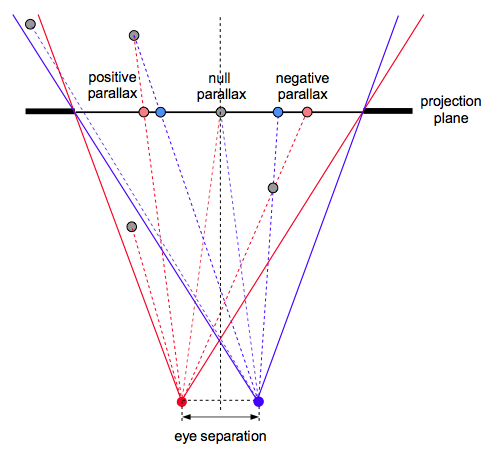
\includegraphics[scale=0.3]{projektiosnparallaxe.png}
\end{center}
\subsubsection{Symmetrische oder asymmetrische Projektion}
Mit zwei symmetrischen PRojektionen auf zwei nicht parallele Projektionsebenen entstehen vertikale Parallaxen, die vom Gehirn nur schwer fusioniert werden können. Diese können verhindert werden, in dem man zwei asymetrische Projektionen auf eine Projektionsebene mit parallelen Blickrichtungen generiert.
\begin{center}
	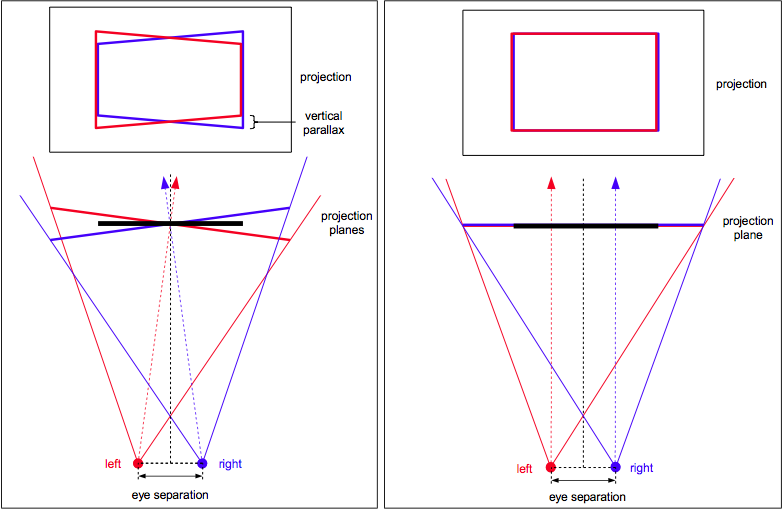
\includegraphics[scale=0.3]{asym-projektion.png}
\end{center}

\subsection{Stereobildübertragung}
Für eine Stereo-Projektion müssen wir nun zwei Bilder generieren und übertragen. Grundsätzlich bedeutet dies nun den doppelten Rechenaufwand für die Generierung. Wie und in welchem Format wir zwei Bilder zum Monitor oder Projektor übertragen hängt von der verwendeten Wiedergabetechnik ab.
\begin{description}
	\item[monoPerspective] \hfill \\
		Perspektivische Projektion von einer Kameraposition aus
	\item[monoOrthographic] \hfill \\
		Orthografische PRojektionen von einer Kameraposition aus.
	\item[stereoColor] \hfill \\
		Mit dieser Technik werden die verschiedenen Anaglyphen mit Farbmaskierung realisiert.
	\item[stereoSideBySide] \hfill \\
		Bei ddieser Technik werden das linke und recht eBild mit jeweils der halben Breite nebeneinander in ein Bild gerendert.
	\item[stereoSideBySideP] \hfill \\
		Hier werden beide Bilder in voller Auflösung gerendert und übertragen.
	\item[stereoLineByLine] \hfill \\
		Bei dieser Technik wird das linke Bild nur in den geraden Zeilen und das Rechte in den ungraden Zeilen gerendert. Der Monitor zeigt abwechslungsweise nur das eine oder andere Bild
	\item[stereoColByCol] \hfill \\
		Gleich wie bei stereoLineByLine aber spaltengetrennt.
	\item[stereoCheckerBoard] \hfill \\
		Bei dieser Technik wechseln sich die Bilder in jedem Pixel ab. Dies führt zu einer Schachbrettartigen Aufteilung.
\end{description}

\newpage
\section{Globale Beleuchtungsmodelle}
\subsection{Beleuchtungsgleichung}
\begin{center}
	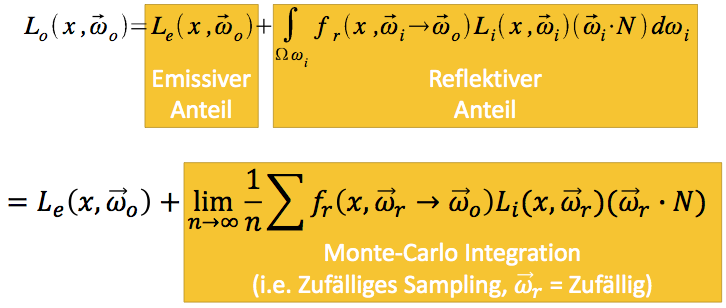
\includegraphics[scale=0.5]{beleuchtungsgleichung.png}
\end{center}

\subsection{Bidirektional Reflectance Distribution Function (BRDF)}
Die BRDF $f_r$ beschreibt bei einem nichttransparenten Material das Verhältnis der von einem Punkt x in Richtung $\overrightarrow{\omega}_r$, ausgehenden differenziellen Strahldichte $L_R$ zur differenziellen Bestrahlungsstärke $E$ die an diesem Punkt aus der Richtung $\overrightarrow{\omega}_i$ ankommt.
\begin{equation}
	f_r(x, \overrightarrow{\omega}_i \rightarrow \overrightarrow{\omega}_r) = \frac{dL_r(\overrightarrow{\omega}_r)}{dL_i(\overrightarrow{\omega}_i)cos(\Theta_i)d\omega_i}
\end{equation}
\begin{center}
	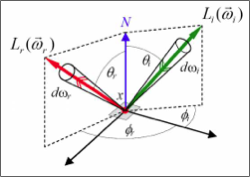
\includegraphics[scale=0.5]{brdf.png}
\end{center}
\subsubsection{Eigenschaften}
\begin{description}
	\item[Reziprozität] \hfill \\
		Eine wichtige Eigenschaft der BRDF ist die Reziprozität die besagt, dass die einfallende Strahlendichte mit der ausfahllenden Strahlendichte vertauscht werden kann. Diese Eigenschaft ist für alle Strahlenverfolgungsalgorithmen von Bedeutung, da es uns erlaubt die Lichtstrahlen vom Auge aus und in ihrer Gegenrichtung zu verfolgen.
	\item[Energieerhaltung] \hfill \\
		Ein Oberflächenpunkt eines passiven Strahlers kann nicht mehr Licht reflektieren, als dort eintrifft. Mit anderen Worten muss das Verhältnis von ausgehender zu ankommender Strahlung kleiner gleich 1 sein.
	\item[Isotropische und anisotropische Reflexion] \hfill \\
		Beim idealen Spiegel liegen die einfallende und ide ausgehende Strahlendichte in einer Ebene und wir sprechen von einer isotropen Reflexion.  Bei vielen manuell bearbeiteten Materialien haben wir eine stark anisotropische und damit gerichtete Reflexion.
\end{description}

\subsection{Lichtweg-Notation}
Die Lichtweg-Notation bezeichnet die Punkte eines Lichtstrahls von der LIchtquelle bis zum Auge mit einer Reihenfolge von Buchstaben. Der Startpunkt bei der Lichtquelle wird $L$ bezeichnet, das Ende beim Auge $E$, eine diffuse Reflexion $D$ und eine spekuläre Reflexion $S$. Für Paare von aufeinanderfolgenden Flächen kann demnach ein Strahl folgende Reflexionsmöglichkeiten haben: diffus-diffus (DD), diffus-spekulär (DS), spekulär-diffus (SD) und spekulär-spekulär (SS).

Ein vollständiger Algorithmus für die globale Beleuchtung müsste jeden Lcihtweg einschliessen, der als $L(D|S)*E$ geschrieben werden kann, wobei ein $|$ oder und ein $*$ kein, ein- oder mehrmals bedeutet.
\begin{center}
	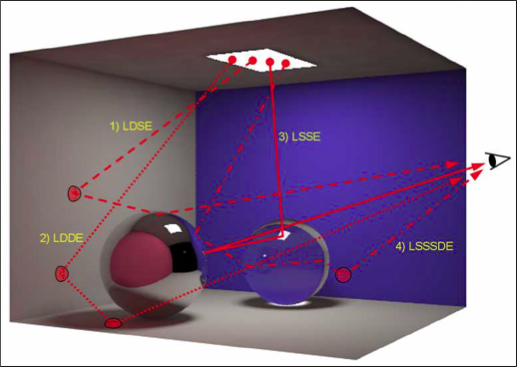
\includegraphics[scale=0.5]{lichtweg-notation.png}
\end{center}

\newpage
\section{Ray Tracing}
\subsection{Photon Tracing}
Dabei werden Photonen per Zufall in einer Szene verfolgt. Trefen die Photonen eine oberfläche, so wird mit einem zweiten Strahl getestet, ob der Schnittpunkt vom Auge aus sichtbar ist.
\begin{center}
	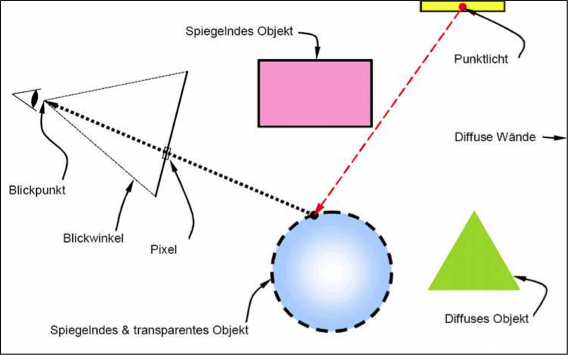
\includegraphics[scale=0.4]{photon-tracing.png}
\end{center}

\subsection{Raytracing}
Die Strahlen werden com Auge ausgehend durch ein Pixel des Bildes in die Szene verfolgt. Trifft ein Strahl auf ein reflektierendes Objekt, so wird ein gespiegelter Strahl weiterverfolgt. Ist das Objekt transparent, so wird ein gebrochener Strahl weiterverfolgt. Diese neuen Strahlen werden rekursiv, mit derselben Funktion behandelt, wie der vom Auge ausgehende Strahl. Die Strahlenverfolgung wird abgebrochen, wenn:
\begin{itemize}
	\item Der Strahl auf den Hintergrund trifft
	\item Der Strahl auf eine rein diffuse Oberfläche trifft
	\item Die Rekursionstiefe einen Maximalwert erreicht
	\item Die Strahlenbeitragskraft einen Minimalwert unterschreitet
\end{itemize}

\begin{center}
	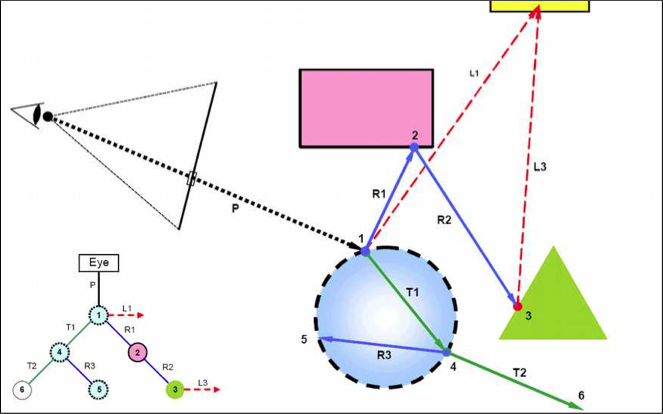
\includegraphics[scale=0.4]{raytracing.png}
\end{center}

Zur Berechnung der Farbintensität muss von jedem Sichtpunkt aus zusätzlich ein sogenannter Schattenstrahl zu jeder Lichtquelle geschickt werden. Schneidet dieser auf seinem Weg ein Objekt, dann liegt der betrachtete unkt im Schatten und der Betrag der Lichtquelle wird bei der Beleuchtungsberechnung nicht berücksichtigt.



\subsection{Distributed Raytracing}
Weil RT immer nur einen Primärstrahl, einen reflektierten Strahl, einen gebrochenen Strahl und ein Schattenfühler verschiesst, erhalten wir die perfekt scharfen Bilder. Dies mag reizvoll sein, entspricht aber relativ schlecht der Ralität, wo oft auch diffuse Spiegelungen und Transparenzen sowie Halbschatten vorkommen. Beim Distributet Raytracing werden deshalb immer mehrere Strahlen vom gleichen Typ verschickt und deren Ertrag gemittelt.
\begin{center}
	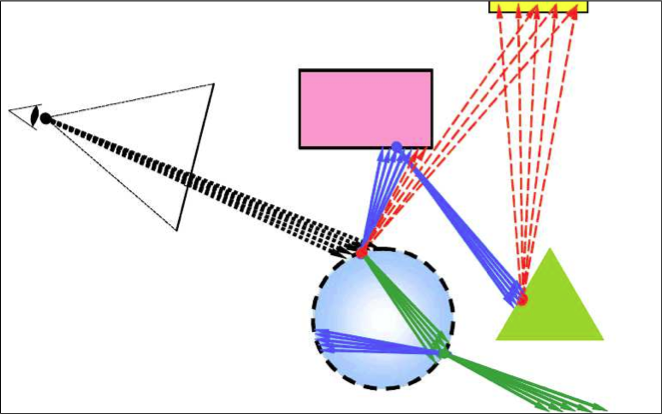
\includegraphics[scale=0.4]{distributed-raytracing.png}
\end{center}
\subsubsection*{Mehrfache Primärstrahlen}
\begin{description}
	\item[Antialiasing] \hfill \\
		Verschickt man mehrere Primärstrahlen vom Blickpunkt durch verschiedene Orte des Pixels, so kann man die erhaltenen Farbwerte mitteln und erreicht dadurch ein Antialiasing
	\item[Motion Blur (Bewegungsunschärfe)] \hfill \\
		Verschickt man mehrere PRimärstrahlen durch ein Pixel, während man ein Objekt verschiebt, so kann man eine Bewegungsunschärfe erzeugen.
	\item[Depth of Field (Tiefenunschärfe)] \hfill \\
		Verschiesst man mehrere PRimärstrahlen von einer Linsenscheibe durch einen Punkt auf der Schärfenebene, so kann man Tiefenunschärfe realisieren.
\end{description}
\subsubsection*{Mehrfache Sekundärstrahlen}
Um unscharfe Spiegelungen und Transparenzen zu erhalten, verschiesst man mehrere reflektierte bzw. gebrochene Strahlen. Die Unschärfe wird ruch das Mass der Abweichung von der perfekten Reflexions- bzw. Transmissionsrichtung bestimmt.
\subsubsection*{Mehrfache Schattenfühler}
Sobald sich in der Szene sichtbare Lichtquellen mit einem Volumen befinden, wirken scharfe Schattenränder schnell unrealistisch. Dort wo nur ein Bereich der Lichtquelle sichtbar ist, entsteht ein Teilschatten. Vom kompletten Schatten bis zur kompletten Beleuchtung entsteht so ein weicher Übergang.

\subsection{Radiosity}
Im ersten Schritt wird vom Blickpunkt unabhängig der Austausch der Strahlungsstärke, beginnend bei selbstrahlenden Patches der Lichtquellen und allen anderen Patches berechnet. Dabei wird nur die rein diffuse Reflexion berücksichtigt.  Nachdem der Strahlungsaustausch von allen Lichtpatches berechnet wurde, geht der Algorithmus der Stärke nach durch alle bestrahlten Patches. Am Schluss des ersten Schrittes weiss jeder Patch seine direkte und indirekte Bestrahlungsstärke. Im zweiten Schritt kann das Bild gerendert werden, indem für jedes Pixel die Radiosity der sichtbaren Patches interpoliert zurückgegeben wird.

Der Vorteil de sRadiosity Algorithmus ist seine relativ effiziente Berechnung der indirekten Beleuchtung, die aus der diffus-diffusen Reflexion kommt. Man hat viel Forschungsaufwand in diesen Algorithmus investiert, weil in der Innenraumbeleuchtungssimulation der gröstte Teil aus dieser Reflexion stammt.
\begin{center}
	\includegraphics[scale=0.4]{radiosity.png}
\end{center}

\subsection{Path Tracing}
Dies ist der erste Algorithmus der einen vollständigen globalen Beleuchtungsalgorithmus besitzt. Beim Path Tracing wird bei jedem Schnittpunkt nur ein Strahl so lange weiterverfolgt, bis er entweder absobiert wird oder in einer Lichtquelle endet. Im Unterschied zum RT werden im PathTracing auch diffus reflektierte Strahlen weiterverfolgt. Um für ein Pixel die korrekte Farbe zu erhalten, müssen viele Pfade verfolgt werden, deren ertrag am Schluss gemittelt wird.
\begin{center}
	\includegraphics[scale=0.4]{pathtracing.png}
\end{center}
\subsubsection{Schnittpunkt Behandlung}
Was bei einem Schnittpunkt passiert, wird mit einer Zufallsvarialen zwischen 0 und 1 entschieden. Je nach Zufallszahl und den Reflexionskoefizienten wird der Strahl diffus reflektiert, spekulär reflektiert, gebrochen oder absobiert. Bei den Reflexionskoeffizienten handelt es sich um Wahrscheinlichkeiten zwischen 0 und 1, die man bei RGB-Koeffizienten durch Drittelung der summierten Komponenten bekommt.
\subsubsection{Lösen der Rendering-Gleichung durch Monte-Carlo Integration}
Wo durch das Pixen ein Primärstrahl geschossen wird oder in welche Richtung ein Strahl reflektiert oder gebrochen wird, wird ebenfalls anhand von Zufallszahlen bestimmt. Mathematisch gesehen entspricht das Abtasten durch zufällige Lichtpfade dem Lösen der Rendering-Gleichung durch Monte Carlo Integration. Diese Technik kann zum Lösen von komplexen Integralen verwedet werden.

\subsection{Bidirektionales Path Tracing}
Die Idee dahinter ist, dass gewisse Lichtpfade besser von der Lichtquelle aus verfolgt werden, anstatt vom Auge aus. Die sgilt insbesondere für PFade die für Lichtbündelungen verantwortlich sind. Das PRoblem ist, dass die Wahrscheinlichkeit mit der ein Strahl bei der diffusen Reflexion in Richtung der ersten spekulären Reflexion geleitet wird, sehr klein ist. Bei der diffusen Reflexion kann der Strahl per Zufall in alle Himmelsrichtungen reflektiert werden. Um diesen energiereichen Pfad zu finden, bräuchte es daher sehr viele Samples und auch dan wären die Lichtbündelungen noch starkt verrauscht. In umgekehrter Richtung ist die Wahrscheinlichkeit des Pfades aber sehr hoch, da er bei den spekulären Reflexionen kaum abweichen kann.

Obwohl bidirektionales PAth Tracing Lichtbündelungen besser erzuegen kann als reines Path Tracing, so leidet die bidirektionale Variante in vielen Fällen immer noch unter Rauschen.

\subsection{Photon Mapping}
Der Algorithmus erhält seinen Namen durch eine Datenstruktur in der Photonen unabhängig von der Geometrie der Objekte gespeichert und gesucht werden können. Er ist in zwei durchgänge aufgeteilt:
\begin{description}
	\item[Photon Tracing] \hfill \\
		Im ersten Durchgang werden Pthotonen von den Lichtquellen in die Szene geschossen. In der Szene interagieren die Photonen mit den vorhandenen Objekten und werden von diesen reflektiert, transmittiert oder absobiert. Beim Auftreffen auf eine diffuse Oberfläche werden die Photonen in der Photonenmap gespeichert.
	\item[Rendering] \hfill \\
		Der zweite Durchgang entspricht dem vom Path Tracer bekannten Rendering. hier wird nun für jeden Schnittpunkt, der auf einer diffusen Oberfläche liegt zusätzlich anhand der im Photon Tracing angelegten Photonmap abgeschätzt wie viel indirektes diffuses LIcht an diesem Punkt angekommen ist.
\end{description}
\subsubsection{Photon Tracing}
Im ersten Durchgang werden die Photonen von den Lichtquellen zufällig in die Szene geschossen nach den physikalischen Eigenschaften der Lichtquellen. Dis geschieht solange bis die gewünschte Anzahl Photonen in der Photonmap gespeichert wurde.

Beim Auftreffen eines Photons auf eine Oberfläche wird anhand der Materialparameter entschieden, ob das Photon diffus reflektiert, spekulär reflektiert, transmittiert oder absorbiert wird. Man spricht hier von Scattering (Streuung), da die Richtung der Reflexion bzw. Transmission, zufällig ermittelt wird. Dieses Vorgehen wird rekursiv solange wiederholt, bis das Photon absorbiert wird. Trifft ein Photon nach mindestens einer Interaktion auf eine diffuse Oberfläche, wird es in der Photonmap gespeichert. Trifft es auf den Hintergrund oder auf eine Lichtquelle, wird es absorbiert. Man beachte, dass Photonen nicht schon bei der ersten diffusen Oberfläche gespeichert werden, da diese die direkte Beleuchtung repräsentieren würden, die im Rendering Durchgang ermittelt wird.
\begin{center}
	\includegraphics[scale=0.4]{photon-scattering.png}
\end{center}

In der Photonmap werden die Photonen gespeichert. Ein Photon ist ein Strahlungsfluss-Träger, dessen Leistung in Watt in den drei Wellenlängenkanlälen RGB untergebracht ist. Die Leistung einer Lichtquelle wird gleichmässig auf die Photonen verteilt. Neben der Leistung müssen zudem Ort und Einfallsrichtung abgespeichert werden.

Während dem Photon-Scattering werden die zu speichernden Photonen einfach in ein Array eingefügt. Danach werden sie in einen sogenannten kd-Baum umgewandelrt. Der Aufwand des Umsortierens ist gerechtfertigt, da die Datenstruktur nur einmal aufgebaut werden muss, die Suche nach den Photonen aber millionenfach stattfindet.
\subsubsection{Rendering}
Im Renderingdurchgang wird mit einem Path Tracer gearbeitet, wobei die Rendering-Gleichung noch Stärker in Teilintegrale aufgeteilt wird.

Zur Berechnung der indirekten Beleuchtung in einem Punkt X der Szene führen wir eine sogenannte Radiance Estimate durch. Diese besteht aus einer Irradiance Estimate und deren Multiplikation mit der BRDF:
\begin{equation}
	L_0(x, \overrightarrow{\omega}_0) = \int_{\Omega_i} f_r(x, \overrightarrow{\omega}_P \rightarrow \overrightarrow{\omega}_0) L_{i,i}(x,\overrightarrow{\omega}_P)(N \bullet\overrightarrow{\omega}_P)d\overrightarrow{\omega}_0
\end{equation}
worin $\overrightarrow{\omega}_0$ die Richtung ist aus der das Photon bei X eintrifft und $L_{i,i}(x,\overrightarrow{\omega}_P)$ die Strahlendichte des einzelnen Photons.

Der Fluss  $\Phi$, der auf die Fläche A trifft, repräsenteirt eine Bestrahlungsstärke (Irradiance). Betrachten wir dazu die Kreisfläche mit $A=\pi r^2$, auf die der Fluss eintrifft. Das Aufsummieren der Flussbeträge der einzelnen Photonen innerhalb des Radius $r$ ergibt den gesammten Fluss auf der Fläche A. Dividiert man durch die Flcähe A, erhält man die ausgehende Strahlenstärke:
\begin{equation}
	L(x,\overrightarrow{\omega}_0) \approx \frac{1}{\pi r^2} \sum_{p=1}^n f_r(x, \overrightarrow{\omega}_P \rightarrow \overrightarrow{\omega}_0) \Phi_P(x, \overrightarrow{\omega}_0)
\end{equation}
mit $n$ im Suchradius $r$ gefundenen, nächstliegenden Photonen.
\begin{center}
	\includegraphics[scale=0.4]{gefundene-photonen.png}
\end{center}

\newpage
\section{RayTracing Verbesserungen}
\subsection{Irrandiance Caching}
\begin{itemize}
	\item Benachbarte Raumpunkte mit ähnlicher Normale werden ähnlich Beleuchtet
	\item Nicht für jedes Pixel die globale Beleuchtung neu berechnen
\end{itemize}
\begin{center}
	\includegraphics[scale=0.3]{IrrandianceCaching.png}
\end{center}

\subsection{Light Cuts}
Dies ist Final Gethering Verfahren, um Szenen mit enorm vielen Punktlichtern effizient zu rendern. Alle Punkte zu verwenden ist zu zeitaufwändig, daher wird eine Herachie der Punkte generiert. Beim Final Gethering wird die Punkthierarchie traversiert und pro Knoten entschieden, ob dieser als Sender verwendet werden kann oder weiter unterteilt werden muss, da der resultierende Fehler zu gross wird. Pro Pixel im Bild wird also ein individueller Cut durch die Hierarchie gebildet.

Als Sender werden nur Knoten aus dem Cut verwendet, dadurch werden es deutlich weniger Punkte. Die Knoten im Cut werden in einer Priority Queue gespeichert. Der Knoten mit der grössten zu erwartenden Änderung wird aus der Queue entnommen und durch seine beiden Kinder ersetzt.
\begin{center}
	\includegraphics[scale=0.3]{lightcut.png}
\end{center}

\subsection{Raumunterteilung}
Die Grundidee der Raumunterteilung liegt wiederum in der Reduktion der potenziellen Schnittpunkttests. Der Raum und damit  die Anzahl Objekte werden dabei so verkleinert, dass nur noch wenige Objekte in einer Raumzelle als Schnittpunktkandidaten infrage kommen. Bei der Verfolgung entlang eines Strahls werden nur noch jende Raumzellen betrachtet, durch die ein Strahl geht. 

Es haben sich verschiedene Unterteilungsstrategieen entwicklet, die je nach Objektdichte und Verteilung besser oder weniger gut geeinget sind.
\begin{center}
	\includegraphics[scale=0.5]{raumunterteilung.png}
	\includegraphics[scale=0.5]{schnitttest.png}
\end{center}

\subsection{Ray Marching}
Schnitttests bei RayTracing sind aufwändig. Alternative: Ray Marching, bei dem nicht ein Schnitttest durchgeführt wird, sonder beim abgeschossenen Strahl in einem definierten Abstand t geprüft wird, ob der Punkt auf dem Strahl innerhalb einer Geometrie liegt oder nicht. Um diesen Test durchzuführen, braucht jedes Objekt eine Distance Field.\\
Definition Distance Field: Funktion, die für jeden Raumpunkt die Distanz zum nächsten Oberflächenpunkt berechnet. Dabei kann diese Funktion signed oder unsigned sein. Der Unterschied zwischen signed und unsigned liegt darin, dass, falls der Punkt auf dem Strahl innerhalb der Geometrie liegt, die Distanzfunktion negativ wird.\\
Um ein Objekt darzustellen braucht es nichts weiteres als eine Distance Field Funktion. Geometrie oder Oberfläche eines Objektes müssen somit nicht definiert werden.\\
Beispiel Distance Field einer Sphere: float sdSphere( vec3 p, float s ) { return length(p)-s; }\\
Erklärung Beispiel: p ist der Punkt, der beim Ray Marching berechnet wurde und s die Grösse der Sphere. Die Berechnung wird dabei im Ursprungspunkt durchgeführt. Das heisst die Sphere sowie ein Ende des Vektors p liegt im Ursprungspunkt. Falls die Länge des Ortsvektors p kleiner ist als der Radius der Sphere, liegt p innerhalb der Sphere.\\
Berechnung t: t wird immer um die Distanz erhöht, die mit per Distance Field berechnet wurde.\\
Schattierung: Ambient Occlusion kann berechnet werden, indem vom Punkt, der bei der Ray Marching berechnet wurde ein Strahl Richtung Lichtquelle geschickt wird.


% Inhalt Ende 
\end{document} 